
\newcommand{\ANIMATEGRAPHICS}[5]{\animategraphics[#1]{#2}{#3}{#4}{#5}}
%\newcommand{\ANIMATEGRAPHICS}[5]{ANIMATION: #3}

%========================================================================
% UNCOMMENT TO PRINT
%========================================================================

% \newcommand{\PAUSE}{}
% \newcommand{\enhance}[1]{}
% \newcommand{\enhancebf}[2]{\textbf{#2}}
% \newcommand{\enhanceus}[1]{\color{blue}}
% \newcommand{\enhancenewus}[1]{\color{magenta}}
% \newcommand{\enhancethem}[1]{\color{red!50!black}}
% \newcommand{\ENHANCE}[1]{
%  \temporal<#1>{\color{lightgray}}{\color{black}}{\color{gray}}}

%========================================================================
% UNCOMMENT FOR PRESENTATION:
%========================================================================

\newcommand{\PAUSE}{\pause}
\newcommand{\enhance}[1]{\temporal<#1>{\color{lightgray}}{\color{black}}{\color{black}}}
\newcommand{\enhancebf}[2]{\enhance{#1}\textbf{#2}}
\newcommand{\enhanceus}[1]{\temporal<#1>{\color{lightgray}}{\color{blue}}{\color{blue}}}
\newcommand{\enhancenewus}[1]{\temporal<#1>{\color{lightgray}}{\color{magenta}}{\color{magenta}}}
\newcommand{\enhancethem}[1]{\temporal<#1>{\color{lightgray}}{\color{red!50!black}}{\color{red!50!black}}}
\newcommand{\ENHANCE}[1]{
\temporal<#1>{\color{lightgray}}{\color{black}}{\color{black}}}
%========================================================================

% UNCOMMENT FOR HANDOUT 
%\documentclass[xcolor=table,slidestop,compress,handout]{beamer}
% UNCOMMENT FOR PRESENTATION
\documentclass[xcolor=table,slidestop,compress]{beamer}

%\documentclass[xcolor=table,compress]{beamer}

\DeclareFontShape{OT1}{cmtt}{bx}{n}{<5><6><7><8><9><10><10.95><12><14.4><17.28><20.74><24.88>cmttb10}{}
\usepackage{mathtools}

\DeclarePairedDelimiter\abs{\lvert}{\rvert}%
\DeclarePairedDelimiter\norm{\lVert}{\rVert}%

%----------------------------------------------------------------------
% For TIKZ flow chart diagrams
\usepackage[latin1]{inputenc}
\usepackage{tikz}
\usetikzlibrary{shapes,arrows}
%----------------------------------------------------------------------

\usepackage[T1]{fontenc}
\usepackage{listings}
\usepackage{bm}
\usepackage{alltt}
\usepackage[overlay]{textpos}
%\usepackage{MnSymbol,wasysym}  % MnSymbol breaks |x|
\usepackage{wasysym}
\usepackage{animate}
\usepackage{minted}
\usepackage[small]{eulervm}
\usepackage{fancybox}
\usepackage{hyperref}

%\usepackage{sphinx}


%\usetheme{Copenhagen}
\usetheme{Luebeck}
%\usetheme{Szeged}
%\usetheme{Montpellier}
%\usetheme{Madrid}
%\usetheme{Warsaw}
%\usetheme{CambridgeUS}

%\useinnertheme{default}
\useoutertheme{infolines}

\newcommand{\icon}{\large{$\bigtriangleup$}}
%\logo{\hfill\hyperlink{titlepage<1>}{\icon}}
%\usecolortheme{default}
%\usecolortheme{sidebartab}
\setbeamersize{text margin left = 0.25in}
%\setbeamercolor{structure}{fg=cyan!90!black}
\usecolortheme{spruce} 
%\usecolortheme{lily} 
%\usecolortheme{dove} % black and white

\newcommand{\etc}{\vspace{-0.05in}\centerline{\dots}\vspace{-0.10in}}
\newcommand{\todo}{$\bigcirc$}

\newcommand{\BUTTON}[1]{#1}
\newcommand{\link}[2]{\hyperlink{#1}{
\includegraphics[height=0.1in]{icon-link.png}\underline{\greentext{#2}}}}


%\newcommand{\sINTRO}{Enzo-P / Cello Project Summary}

%==================================================
\newcommand{\ssPurpose}{What is the purpose of this document?}

%==================================================
\newcommand{\sIntro}{What is Enzo-P/Cello?}
\newcommand{\ssMotivation}{Why does Enzo-P exist?}
\newcommand{\ssAmr}{How does Enzo-P's AMR differ from Enzo's?}
\newcommand{\ssCompare}{How do Enzo-P and Enzo differ?}
\newcommand{\ssApproach}{How does Enzo-P address Enzo's limitations?}

\newcommand{\sRecent}{New features}
\newcommand{\ssRecentMusic}{MUSIC initial conditions}
\newcommand{\ssRecentSolvers}{Separate Solvers objects}
\newcommand{\ssRecentScalableGravity}{``Scalable'' AMR gravity}
\newcommand{\ssRecentExpansion}{Cosmological expansion}
\newcommand{\ssRecentCosmology}{``Scalable'' AMR Cosmology}
\newcommand{\ssRecentPpmDevel}{Updated PPM hydrodynamics}
\newcommand{\ssRecentMisc}{Miscellaneous new features}
%@@@@@@@@@@@@@@
\newcommand{\ssRecentParticles}{Abstract particles}
\newcommand{\ssRecentGravity}{Scalable gravity}
\newcommand{\ssRecentHistory}{Old fields}
\newcommand{\ssRecentTemporary}{Temporary fields}

\newcommand{\sSoon}{Coming soon\ldots}
\newcommand{\ssSoonIo}{MUSIC I.C.'s}
\newcommand{\ssSoonYt}{yt support}
\newcommand{\ssSoonUnits}{Units}

%==================================================
\newcommand{\sCharm}{\charm\ system}
\newcommand{\ssCharm}{What is \charm?}
\newcommand{\ssCharmCode}{How do I write a simple \charm\ program?}
\newcommand{\ssCharmPup}{\charm\ ``pup'' functions--what are they?}
\newcommand{\ssCharmCello}{How is \charm\ used in Cello?}
%==================================================
\newcommand{\sDesign}{Software design}

\newcommand{\ssOop}{Design overview}
\newcommand{\ssComponents}{Cello software components}
\newcommand{\ssClasses}{Enzo-P / Cello classes}
\newcommand{\ssSimulation}{Simulation classes}
\newcommand{\ssProblems}{Problem classes}
\newcommand{\ssBlocks}{Block and Data classes}
%\newcommand{\ssData}{The Data class}
\newcommand{\ssFields}{Field data classes}
\newcommand{\ssParticles}{Particle data classes}
\newcommand{\ssMethods}{Method classes}
\newcommand{\ssInitialBoundary}{Initial and Boundary conditions classes}
\newcommand{\ssRefine}{Mesh refinement criteria classes}
%\newcommand{\ssStopping}{Stopping criteria class}
%\newcommand{\ssClassesOrg}{How are Enzo-P's classes organized?}

%==================================================
\newcommand{\sDevel}{Developing Enzo-P}

%\newcommand{\sCODE}{Enzo-P / Cello Source Code Design and Implementation}
\newcommand{\ssDevelCoding}{Enzo-P develper coding guidelines and suggestions}
\newcommand{\ssDevelParameter}{How do I add a new input parameter?}
\newcommand{\ssDevelMethod}{How do I add a new method?}
\newcommand{\ssDevelFields}{How do I write a Method using Fields?}
\newcommand{\ssDevelParticles}{How do I write a Method using Particles?}
\newcommand{\ssDevelInitial}{How do I add initial conditions?}
\newcommand{\ssDevelBoundary}{How do I add new boundary conditions?}
\newcommand{\ssDevelRefine}{How do I add a new refinement criterium?}
\newcommand{\ssDevelTest}{How do I add a new unit test program?}

%==================================================
\newcommand{\sFuture}{What else needs to be done?}

\newcommand{\ssRoadmap}{What is the project roadmap?}
\newcommand{\ssFutureHydro}{Unfinished business: hydrodynamics}
\newcommand{\ssFutureGravity}{Unfinished business: gravity}
\newcommand{\ssFutureChemistry}{Unfinished business: chemistry}
\newcommand{\ssFutureParticles}{Unfinished business: particles}
\newcommand{\ssFutureMagnetism}{Unfinished business:  MHD}
\newcommand{\ssFutureRadiation}{Unfinished business: radiation}
\newcommand{\ssContribute}{How can I contribute?}

%==================================================
\newcommand{\sParameters}{Parameter files}

\newcommand{\ssParamIntro}{Enzo-P/Cello parameter files}
\newcommand{\ssParameters}{Writing Enzo-P parameter files}
\newcommand{\ssDoubleMach}{Case Study: Double Mach Reflection}
\newcommand{\ssParamActivity}{Getting to know Enzo-P better}

\newcommand{\ssCharmSummary}{Summary}
\newcommand{\ssControlSummary}{Summary}
\newcommand{\ssDesignSummary}{Summary}
\newcommand{\ssDevelSummary}{Summary}
\newcommand{\ssFutureSummary}{Summary}
\newcommand{\ssIntroSummary}{Summary}
\newcommand{\ssParametersSummary}{Summary}
\newcommand{\ssPresentSummary}{Summary}
\newcommand{\ssRecentSummary}{Summary}
\newcommand{\ssProjectSummary}{Summary}
\newcommand{\ssStartingSummary}{Summary}

%\newcommand{\ssParamProblem}{What parameters are available for defining problems?}
%\newcommand{\ssParamRefine}{What parameters are available for controling mesh refinement?}
%\newcommand{\ssParamData}{What parameters are available for defining data structures?}
%\newcommand{\ssParamMethod}{What parameters are available for specifying numerical methods?}
%\newcommand{\ssParamIo}{What parameters are available for controling I/O?}
%\newcommand{\ssParamOther}{What other parameters are available?}

%==================================================
\newcommand{\sControl}{Control flow}

\newcommand{\ssControl}{How are phases of the computation controlled?}
\newcommand{\ssAdapt}{Adaptive Mesh Refinement}
\newcommand{\ssRefresh}{Refresh ghost zones}

%==================================================
\newcommand{\sPresent}{Current status}

\newcommand{\ssState}{What is the current status of Enzo-P/Cello?}
\newcommand{\ssCurrent}{What are Enzo-P's current capabilities?}
\newcommand{\ssScaling}{How well does Enzo-P scale?}
\newcommand{\ssIssues}{What are some of Enzo-P's known issues?}

%==================================================
\newcommand{\sProject}{Project organization}

\newcommand{\ssProject}{How is the Enzo-P project currently organized?}
\newcommand{\ssSource}{How is the source code directory organized?}
\newcommand{\ssBrowse}{How can I browse the source code?}
\newcommand{\ssDocumentation}{What documentation is available?}
\newcommand{\ssBugs}{What are some of the known bugs?}
\newcommand{\ssTesting}{How is testing done?}
%\newcommand{\ssCommunicate}{How do Enzo-P developers communicate?}

%==================================================
\newcommand{\sStarting}{Getting started}

\newcommand{\ssStarting}{Getting started using Enzo-P / Cello}
\newcommand{\ssInstallCharm}{How do I download and install Charm++?}
\newcommand{\ssInstallEnzop}{How do I download Enzo-P?}
\newcommand{\ssConfigure}{How do I configure Enzo-P?}
\newcommand{\ssCompile}{How do I compile Enzo-P?}
\newcommand{\ssRunning}{How do I run an example problem?}
%\newcommand{\ssDoubleMach}{Double Mach Reflection}
\newcommand{\ssRestart}{How do I restart from a checkpoint?}
\newcommand{\ssLoadBalance}{How do I run with dynamic load balancing?}
\newcommand{\ssTools}{What tools does Cello provide?}


%==================================================
\newcommand{\sTemplate}{TEMPLATE SECTION TITLE}
%==================================================

\newcommand{\orow}[1]{\textcolor{blue}{#1}}
\newcommand{\erow}[1]{\textcolor{blue!50!black}{#1}}

\newcommand{\blockred}{\setbeamercolor{block title}{bg=red!30,fg=black}}
\newcommand{\blockgreen}{\setbeamercolor{block title}{bg=green!30,fg=black}}
\newcommand{\blockblue}{\setbeamercolor{block title}{bg=blue!30,fg=black}}

\newcommand{\bad}{\textcolor{red}{\frownie}}
\newcommand{\good}{\textcolor{green}{\smiley}}
\newcommand{\blck}{\code{Block}}
\newcommand{\cello}{\textsf{Cello}}
\newcommand{\charm}{{\sf Charm\pp}}

\newcommand{\code}[1]{\texttt{#1}}


\newcommand{\yellowcode}[1]{\textcolor{yellow!50!black}{\code{#1}}}
\newcommand{\greycode}[1]{\textcolor{grey}{\code{#1}}}
\newcommand{\cyancode}[1]{\textcolor{cyan!50!black}{\code{#1}}}

\newcommand{\urltext}[1]{\greentext{\url{#1}}}
\newcommand{\bluecode}[1]{\textcolor{blue}{\code{#1}}}
\newcommand{\greencode}[1]{\textcolor{green!50!black}{\code{#1}}}
\newcommand{\redcode}[1]{\textcolor{red!50!black}{\code{#1}}}
\newcommand{\magentacode}[1]{\textcolor{magenta}{\code{#1}}}
\newcommand{\purplecode}[1]{\textcolor{purple!70!black}{\code{#1}}}
\newcommand{\orangecode}[1]{\textcolor{orange!60!black}{\code{#1}}}

\newcommand{\greyit}[1]{\textcolor{grey}{\textit{#1}}}
\newcommand{\cyanit}[1]{\textcolor{cyan!50!black}{\textit{#1}}}
\newcommand{\blueit}[1]{\textcolor{blue}{\textit{#1}}}
\newcommand{\greenit}[1]{\textcolor{green!50!black}{\textit{#1}}}
\newcommand{\redit}[1]{\textcolor{red!50!black}{\textit{#1}}}
\newcommand{\magentait}[1]{\textcolor{magenta!70!black}{\textit{#1}}}
\newcommand{\orangeit}[1]{\textcolor{orange!60!black}{\textit{#1}}}

\newcommand{\redtext}[1]{\textcolor{red!70!black}{#1}}
\newcommand{\cyantext}[1]{\textcolor{cyan!50!black}{#1}}
\newcommand{\orangetext}[1]{\textcolor{orange!60!black}{#1}}
\newcommand{\yellowtext}[1]{\textcolor{yellow!50!black}{#1}}
\newcommand{\greentext}[1]{\textcolor{green!50!black}{#1}}
\newcommand{\bluetext}[1]{\textcolor{blue}{#1}}
\newcommand{\magentatext}[1]{\textcolor{magenta!70!black}{#1}}

\newcommand{\addclass}[1]{\bluetext{#1}}
\newcommand{\addconstruct}[1]{\cyantext{#1}}
\newcommand{\addparam}[1]{\magentatext{#1}}
\newcommand{\addcharm}[1]{\redtext{#1}}
\newcommand{\addtest}[1]{\greentext{#1}}

\newcommand{\addclassbf}[1]{\bluetext{\textbf{#1}}}
\newcommand{\addconstructbf}[1]{\cyantext{\textbf{#1}}}
\newcommand{\addparambf}[1]{\magentatext{\textbf{#1}}}
\newcommand{\addcharmbf}[1]{\redtext{\textbf{#1}}}
\newcommand{\addtestbf}[1]{\greentext{\textbf{#1}}}

\newcommand{\redcirc}{\textcolor{red!50!black}{$\bigcirc$}}
\newcommand{\orangecirc}{\textcolor{orange!60!black}{$\bigcirc$}}
\newcommand{\yellowcirc}{\textcolor{yellow!50!black}{$\bigcirc$}}
\newcommand{\greencirc}{\textcolor{green!50!black}{$\bigcirc$}}
\newcommand{\bluecirc}{\textcolor{blue}{$\bigcirc$}}
\newcommand{\magentacirc}{\textcolor{magenta!70!black}{$\bigcirc$}}


\newcommand{\redbf}[1]{\textcolor{red!50!black}{\textbf{#1}}}
\newcommand{\cyanbf}[1]{\textcolor{cyan!50!black}{\textbf{#1}}}
\newcommand{\orangebf}[1]{\textcolor{orange!60!black}{\textbf{#1}}}
\newcommand{\yellowbf}[1]{\textcolor{yellow!50!black}{\textbf{#1}}}
\newcommand{\greenbf}[1]{\textcolor{green!50!black}{\textbf{#1}}}
\newcommand{\bluebf}[1]{\textcolor{blue}{\textbf{#1}}}
\newcommand{\magentabf}[1]{\textcolor{magenta!70!black}{\textbf{#1}}}

\newcommand{\highpriority}{}
\newcommand{\medpriority}{}
\newcommand{\lowpriority}{}

\newcommand{\group}[1]{\bluecode{#1}}
\newcommand{\subgroup}[1]{\greencode{#1}}
\newcommand{\parameter}[1]{\redcode{#1}}
\newcommand{\valuetext}[1]{\cyancode{#1}}
\newcommand{\comment}[1]{\textsf{\textbf{\blueit{#1}}}}

\newcommand{\type}[1]{\greencode{#1}}
\newcommand{\variable}[1]{\orangecode{#1}}
\newcommand{\function}[1]{\bluecode{#1}}
\newcommand{\keyword}[1]{\purplecode{#1}}

\newcommand{\enzopcello}{\textsf{Enzo-P/Cello}}
\newcommand{\enzop}{\textsf{Enzo-P}}
\newcommand{\enzo}{\textsf{Enzo}}
\newcommand{\itemnum}[1]{\item<#1>}
\newcommand{\newus}[1]{\color{magenta!70!black}{#1}}
\newcommand{\patch}{\code{Patch}}
\newcommand{\pp}{\texttt{++}}
\newcommand{\seed}{\code{Seed}}
\newcommand{\seedgrid}{\code{SeedGrid}}
\newcommand{\seedtree}{\code{SeedTree}}
\newcommand{\them}[1]{\color{red!50!black}{#1}}
\newcommand{\tree}{\code{Tree}}
\newcommand{\us}[1]{\color{blue}{#1}}
\newcommand{\cursor}[1]{\uncover<#1>{\begin{animateinline}[autoplay,loop]{2.0}
\strut\textbf{\_}\newframe\newframe[5]
\end{animateinline}}}
\newcommand{\prompt}{\textcolor{blue!50!black}{\$}}
\newcommand{\bfat}[2]{\alt<#1>{\textbf{#2}}{#2}}
%\newcommand{\colorat}[2]{\textcolor<#1>{f{#2}}{#2}}
\newcommand{\TITLE}[2]{\title{#1}
\subtitle{#2}
\author[Bordner/Norman]{James Bordner \and Michael L.~Norman}
\institute {
   University of California, San Diego\\
   San Diego Supercomputer Center}
\date[2018-05-14/18]{Enzo Days 2018 / Georgia Tech \\
            2018-05-14/18}}

\definecolor{enzop}{rgb}{0.75,0.00,0.00}
\definecolor{cello}{rgb}{0.00,0.50,0.000}


% background color
% \beamersetaveragebackground{yellow!10}
\beamertemplatetransparentcoveredhigh
%\beamertemplatetransparentcovereddynamicmedium
%@@@@@@@@@@@@@@@@@@@@@@@@@@@@@@@@@@@@@@@@@@@@@@@@@@
% This removes paretheses around ``name (institution)'' in footer
%@@@@@@@@@@@@@@@@@@@@@@@@@@@@@@@@@@@@@@@@@@@@@@@@@@
\makeatletter
\setbeamertemplate{footline}
{
  \leavevmode%
  \hbox{%
  \begin{beamercolorbox}[wd=.333333\paperwidth,ht=2.25ex,dp=1ex,center]{author in head/foot}%
    \usebeamerfont{author in head/foot}\insertshortauthor%~~\beamer@ifempty{\insertshortinstitute}{}{(\insertshortinstitute)}
  \end{beamercolorbox}%
  \begin{beamercolorbox}[wd=.333333\paperwidth,ht=2.25ex,dp=1ex,center]{title in head/foot}%
    \usebeamerfont{title in head/foot}\insertshorttitle
  \end{beamercolorbox}%
  \begin{beamercolorbox}[wd=.333333\paperwidth,ht=2.25ex,dp=1ex,right]{date in head/foot}%
    \usebeamerfont{date in head/foot}\insertshortdate{}\hspace*{2em}
    \insertframenumber{} / \inserttotalframenumber\hspace*{2ex} 
  \end{beamercolorbox}}%
  \vskip0pt%
}
\makeatother




\begin{document}

%======================================================================
\TITLE{Enzo-P / Cello Status and What's New?}{ \ \\
%======================================================================
\tiny{NSF SI2-SSE-1440709 PHY-1104819 AST-0808184}}

\frame[label=titlepage]{ \titlepage }

%\setbeamertemplate{frametitle}{%
%\begin{beamercolorbox}[wd=\textwidth, ht=0.5cm, dp=0.2cm]{frametitle}
%\usebeamerfont{frametitle}\insertframetitle
%\end{beamercolorbox}}

\newcommand{\modframetitle}[1]{\frametitle{(\arabic{ModuleCounter}) #1 }}
\newcommand{\secframetitle}[1]{\frametitle{(\arabic{ModuleCounter}.\arabic{SectionCounter}) #1 }}

\newcounter{ModuleCounter}
\newcommand{\NEWMOD}{\stepcounter{ModuleCounter}\setcounter{SectionCounter}{0}}
\newcounter{SectionCounter}
\newcommand{\NEWSEC}{\stepcounter{SectionCounter}}


%======================================================================
% TOP LEVEL MENU
%======================================================================
\begin{frame}[fragile,label=outline] 
\frametitle{Chapters}
\begin{center}
\begin{minipage}{3.25in}
\begin{enumerate}
%--------------------------------------------------
\item  \hyperlink{s-intro<1>}      {\BUTTON {\orow{\sIntro}}} \\
\item  \hyperlink{s-project<1>}    {\BUTTON {\erow{\sProject}}} \\
\item  \hyperlink{s-present<1>}    {\BUTTON {\orow{\sPresent}}} \\
\item  \hyperlink{s-recent<1>}     {\BUTTON {\erow{\sRecent}}} \\
\item  \hyperlink{s-future<1>}     {\BUTTON {\orow{\sFuture}}} \\
%\item  \hyperlink{s-starting<1>}   {\BUTTON {\orow{\sStarting}}} \\
%\item  \hyperlink{s-parameters<1>} {\BUTTON {\erow{\sParameters}}} \\
%\item  \hyperlink{s-charm<1>}      {\BUTTON {\orow{\sCharm}}} \\
%\item \hyperlink{s-design<1>}      {\BUTTON {\erow{\sDesign}}} \\
%\item \hyperlink{s-control<1>}      {\BUTTON {\orow{\sControl}}} \\
%\item  \hyperlink{s-devel<1>} {\BUTTON {\erow{\sDevel}}}
%\end{tabular}
\end{enumerate}
\end{minipage}
\end{center}
\end{frame}


%======================================================================
\NEWMOD \section{\sIntro}
%======================================================================

%----------------------------------------------------------------------

\logo{\hfill\hyperlink{outline<1>}{\icon}}

\begin{frame}[fragile,label=s-intro] 
\modframetitle{\sIntro}
\small
\begin{center}
\begin{minipage}{3.25in}
\begin{enumerate}
%\item \hyperlink{ss-purpose<1>}   {\BUTTON {\ssPurpose}}
\item \hyperlink{ss-motivation<1>} {\BUTTON {\ssMotivation}}  % 1.1
\item \hyperlink{ss-amr<1>}        {\BUTTON {\ssAmr}}          % 1.2
\item \hyperlink{ss-charm<1>}      {\BUTTON {\ssCharm}}          % 1.2
\item \hyperlink{ss-compare<1>}    {\BUTTON {\ssCompare}}      % 1.3
%\item \hyperlink{ss-approach<1>}   {\BUTTON {\ssApproach}}     % 1.5
\item \hyperlink{ss-intro-summary<1>}   {\BUTTON {\ssIntroSummary}}
\end{enumerate}
\end{minipage}
\end{center}
\end{frame}

\logo{\hfill\hyperlink{s-intro<1>}{\icon}}

%%======================================================================
\NEWSEC
%======================================================================

%\subsection{\ssPurpose}

\begin{frame}[fragile,label=ss-purpose] 
\frametitle{\ssPurpose}

Three main goals:
\begin{enumerate}
\item Tell you \blueit{\textbf{what} Enzo-P is} (and \blueit{\textbf{why} it exists})
\item Help you learn to \blueit{\textbf{use} Enzo-P}
\begin{itemize}
\item download Enzo-P / Cello
\item configure / compile / run
\item write parameter files
\end{itemize}
\item Show you how to \blueit{\textbf{develop} Enzo-P}
\begin{itemize}
\item \charm\ parallel programming system
\item Cello software design
\item add parameters
\item add methods, refinement criteria
\item add initial and boundary conditions
\end{itemize}
\end{enumerate}
%Enzo-P has had a single developer for long enough. \\
%That needs to change. \\
%Today! \pause (\ldots and tomorrow)
\end{frame}

%Other material that needs to be covered:
%\begin{itemize}
%\item \blueit{Charm++} Parallel programming system
%\item Current \blueit{project organization}
%\end{itemize}
    % What is the purpose of this workshop?

%----------------------------------------------------------------------
\NEWSEC \subsection{\ssMotivation}
%----------------------------------------------------------------------
%\begin{frame}[fragile,label=ss-motivation] 
\secframetitle{\ssMotivation}
% One might ask why am I working on Enzo-P and Cello.  Enzo is clearly
% a very powerful code, capable of being applied to a wide range
% of problems in astrophysics and cosmology.

% [PHYSICS] This is due in part to Enzo's wide range of physics
% capabilites, from hydrodynamics and self-gravity, to cosmological
% expansion, chemistry and cooling, star formation, MHD, RHD, and so
% on.

% [METHODS] Enzo contains an even wider range of numerical methods,
% which serve to discretize and solve these equations.  Most of the
% physics capabilities in Enzo can be solved using one of multiple
% available methods, such as PPM, ZEUS or MUSCL hydrodynamics,
% Gadget, Cloudy, and Grackle chemistry and cooling, and implicit
% coupled FLD and Enzo+Moray RHD

% [DATA] All of Enzo's methods are in turn built on its parallel
% adaptive mesh refinement data structure.  Patches in the AMR
% hierarchy contain both particle data and mesh data, so both
% Lagrangian and Eularian methods are supported, as well as hybrid
% particle-mesh methods.

% [SLIDE] Together, these three layers enable Enzo to do numerical
% astrophysics.  The equations serve to mathematically approximate
% physical phenomena, the numerical methods serve to define how to
% represent required data on a computer and proceedures for finding
% numerical solutions to the equations, and the data structures serve
% to represent the actual numerical solution including all
% intermediate computations within the parallel computer.
  \framesubtitle{\enzo's strengths}
\centerline{\textbf{\only<1>{Applicable to a wide range of astrophysical/cosmological problems}
\only<2>{Implements a variety of sophisticated numerical methods}
\only<3>{Enabled by adaptive mesh refinement with particles and fields}}}
\setbeamercolor{block title}{bg=red!30,fg=black}
\begin{block}<+->{\textbf{Physics Equations}: \textit{mathematical models}}
   \textcolor{red!80!black}{
 \footnotesize
    \textbullet\ Hydrodynamics (Euler equations)
    \textbullet\ Gravity ($\nabla^2\Phi=4\pi G\rho$)
    \textbullet\ Chemistry/cooling
    \textbullet\ Star formation
    \textbullet\ Magnetism
    \textbullet\ Radiation \Large $\ldots$
    }
\end{block}

\setbeamercolor{block title}{bg=green!30,fg=black}
\begin{block}<+->{\textbf{Numerical Methods}: \textit{approximate and solve}}
    \textcolor{green!50!black}{
\footnotesize     \textbullet\ PPM, \textbullet\ ZEUS, \textbullet\ MUSCL
     \textbullet\ FFT \textbullet\ multigrid
     \textbullet\ Gadget cooling
     \textbullet\ Cloudy cooling
     \textbullet\ Grackle
     \textbullet\ Dedner MHD
     \textbullet\ MHD-CT
     \textbullet\ Implicit FLD
     \textbullet\ Moray \Large $\ldots$
     }
  \end{block}

\setbeamercolor{block title}{bg=blue!30,fg=black}
\begin{block}<+->{\textbf{Data Structures}: \textit{computer representation}}
    \textcolor{blue}{
\footnotesize
    \textbullet\ Structured Adaptive Mesh Refinement (SAMR)
    \textbullet\ Eularian fields
    \textbullet\ Lagrangian particles
 \Large $\ldots$}
  
\end{block}

\end{frame}

%-----------------------------------------------------------------------

 \begin{frame}[fragile] 

% The main thing that Enzo struggles with is keeping up with
% the continual exponential increase in parallelism in HPC
% systems.  20 years ago when Enzo was first conceived,
% typical ``massively parallel'' machines had on the order
% of 100 processors, but today's machines have thousands times
% more cores.

% The physics is relatively untouched.  We still want to solve the
% same equations we did 20 years ago.  The numerical methods are also
% mostly the same--hydrodynamics/chemistry are local, FFT's and
% multigrid require some changes but still viable.  The main effect is
% on Enzo's parallel AMR data structures.  AMR meta data didn't used
% to be a problem, but it's a hard limit on scalability now.
% Hierarchy overhead wasn't a problem when it had to loop over
% hundreds of grids, but now it is when it has to loop over millions.
% As hardware parallelism increases, Enzo runs into bottleneck after
% bottleneck, in both memory usage and parallel computation.  Even MPI
% as used in Enzo has limits---barriers and other global operations
% become increasingly costly as core counts increase

% This is what motivated me to start working on Enzo-P/Cello.
% The idea was to redesign and implement the AMR data structure
% from scratch to be as scalable as possible, targeting machines
% that didn't even exist when the project started.  This AMR
% data structure is in a separate reusable framework called Cello.
% Enzo-P is the port of Enzo's physics and numerical methods onto
% Cello.

%---------
% SLIDE 2
%---------

% That's a summary of Enzo's strengths.  Enzo has limitations as well,
% and they are primarily due to the vast increase in size and
% complexity of the high performance computer hardware we have access
% to.  Development on Enzo began about 20 years ago, when ``massively parallel''
% meant about 100 processors.  Today, supercomputers can contain
% a hundred *thousand* processors.  This has affected the three conceptual layers of 
% Enzo in different ways.

% [PHYSICS] The higher-level mathematical equations defining the physics
% are mostly unchanged.  The equations for hydrodynamics and gravity are the
% same today as they were 20 years ago.  Enzo has certainly increased
% its range of problems it can solve, for example by adding support for MHD and RHD,
% but the existing physics requirements are unchanged.

% [METHODS] Numerical methods in Enzo are still very usable for the
% most part.  Methods for solving localized physics such as
% hydrodynamics and chemistry and cooling have the same requirements
% as 20 years ago, and those for global physics such as self-gravity
% are based on FFT's and multigrid, which are still usable on todays
% supercomputers, though may require some optimizations in terms of
% structuring the data

% [DATA STRUCTURES] Which brings us to data structures.  Of these
% three, supercomputer growth has affected the usability of Enzo's
% data structures the most.  Unfortunately, they're also the most
% difficult to change, since all of Enzo's numerical methods use them,
% and changing any part of how Enzo does AMR can lead to a global
% effect on the code.

% [ENZO-P] This is why several years ago I started working on Enzo-P
% and Cello.  Enzo-P serves to contain the physics capabilities and
% numerical methods in Enzo, whereas Cello serves to implement a
% totally new AMR framework designed to be highly scalable, capable of
% running on petascale and ultimately exascale machines.  Needless to
% say, designing software to run on classes of machines that don't
% exist yet is difficult, though a lot of thought has been put into
% making Cello as scalable as possible, so that Enzo's physics can
% continue to live and thrive for many years to come.

\secframetitle{\ssMotivation}
%  \framesubtitle{\enzo's struggles}
 \centerline{\textbf{ENZO has difficulties scaling to modern HPC platforms}} \ \\
 \begin{minipage}{3in}
\pause
  \begin{itemize}
   \item Ever-changing software requirements
     \begin{itemize}
\footnotesize
   \item  Enzo was born in early 1990's
   \item ``massive parallelism'' meant $P\approx 100$
   \item $\times 10^5$ parallelism today
     \end{itemize}
   
\pause
   \item Affects different parts of \enzo\ differently
     \begin{itemize}
   \item[\smiley] \textcolor{red!80!black}{physics} requirements unchanged
   \item[\smiley] \textcolor{green!50!black}{numerical methods} mostly viable
   \item[\frownie] \textcolor{blue}{\textit{data structures}} limit Enzo's scalability
     \end{itemize}
\pause
   \item Motivates AMR data structure redesign
   \begin{itemize}
   \footnotesize
   \item  \textbf{\enzop}: ``petascale'' version of \enzo
   \item keep \enzo's \textcolor{red!80!black}{physics} and many \textcolor{green!50!black}{methods}
   \item  built on \textbf{\cello} \textcolor{blue}{scalable AMR framework}
   \end{itemize}
  \end{itemize}
\end{minipage}
\begin{minipage}{1in}
   \footnotesize
    \centerline{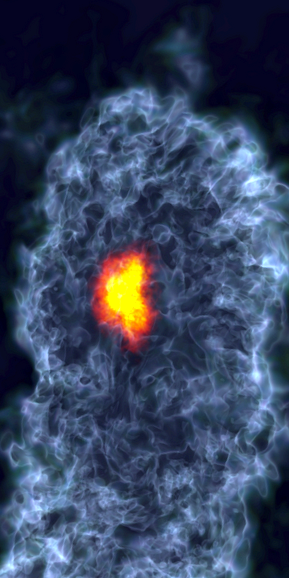
\includegraphics[width=0.875in]{PopIII_vr-edit.png}}
    \centerline{\tiny {[ Sam Skillman, Matt Turk ]}}
\end{minipage}
\end{frame}

%%======================================================================
\NEWSEC
%======================================================================

\subsection{\ssMotivation}

\begin{frame}[fragile,label=ss-motivation] 
\secframetitle{\ssMotivation}
% One might ask why am I working on Enzo-P and Cello.  Enzo is clearly
% a very powerful code, capable of being applied to a wide range
% of problems in astrophysics and cosmology.

% [PHYSICS] This is due in part to Enzo's wide range of physics
% capabilites, from hydrodynamics and self-gravity, to cosmological
% expansion, chemistry and cooling, star formation, MHD, RHD, and so
% on.

% [METHODS] Enzo contains an even wider range of numerical methods,
% which serve to discretize and solve these equations.  Most of the
% physics capabilities in Enzo can be solved using one of multiple
% available methods, such as PPM, ZEUS or MUSCL hydrodynamics,
% Gadget, Cloudy, and Grackle chemistry and cooling, and implicit
% coupled FLD and Enzo+Moray RHD

% [DATA] All of Enzo's methods are in turn built on its parallel
% adaptive mesh refinement data structure.  Patches in the AMR
% hierarchy contain both particle data and mesh data, so both
% Lagrangian and Eularian methods are supported, as well as hybrid
% particle-mesh methods.

% [SLIDE] Together, these three layers enable Enzo to do numerical
% astrophysics.  The equations serve to mathematically approximate
% physical phenomena, the numerical methods serve to define how to
% represent required data on a computer and proceedures for finding
% numerical solutions to the equations, and the data structures serve
% to represent the actual numerical solution including all
% intermediate computations within the parallel computer.
  \framesubtitle{\enzo's strengths}
\centerline{\textbf{\only<1>{Applicable to a wide range of astrophysical/cosmological problems}
\only<2>{Implements a variety of sophisticated numerical methods}
\only<3>{Enabled by adaptive mesh refinement with particles and fields}}}
\setbeamercolor{block title}{bg=red!30,fg=black}
\begin{block}<+->{\textbf{Physics Equations}: \textit{mathematical models}}
   \textcolor{red!80!black}{
 \footnotesize
    \textbullet\ Hydrodynamics (Euler equations)
    \textbullet\ Gravity ($\nabla^2\Phi=4\pi G\rho$)
    \textbullet\ Chemistry/cooling
    \textbullet\ Star formation
    \textbullet\ Magnetism
    \textbullet\ Radiation \Large $\ldots$
    }
\end{block}

\setbeamercolor{block title}{bg=green!30,fg=black}
\begin{block}<+->{\textbf{Numerical Methods}: \textit{approximate and solve}}
    \textcolor{green!50!black}{
\footnotesize     \textbullet\ PPM, \textbullet\ ZEUS, \textbullet\ MUSCL
     \textbullet\ FFT \textbullet\ multigrid
     \textbullet\ Gadget cooling
     \textbullet\ Cloudy cooling
     \textbullet\ Grackle
     \textbullet\ Dedner MHD
     \textbullet\ MHD-CT
     \textbullet\ Implicit FLD
     \textbullet\ Moray \Large $\ldots$
     }
  \end{block}

\setbeamercolor{block title}{bg=blue!30,fg=black}
\begin{block}<+->{\textbf{Data Structures}: \textit{computer representation}}
    \textcolor{blue}{
\footnotesize
    \textbullet\ Structured Adaptive Mesh Refinement (SAMR)
    \textbullet\ Eularian fields
    \textbullet\ Lagrangian particles
 \Large $\ldots$}
  
\end{block}

\end{frame}

%-----------------------------------------------------------------------

 \begin{frame}[fragile] 

% The main thing that Enzo struggles with is keeping up with
% the continual exponential increase in parallelism in HPC
% systems.  20 years ago when Enzo was first conceived,
% typical ``massively parallel'' machines had on the order
% of 100 processors, but today's machines have thousands times
% more cores.

% The physics is relatively untouched.  We still want to solve the
% same equations we did 20 years ago.  The numerical methods are also
% mostly the same--hydrodynamics/chemistry are local, FFT's and
% multigrid require some changes but still viable.  The main effect is
% on Enzo's parallel AMR data structures.  AMR meta data didn't used
% to be a problem, but it's a hard limit on scalability now.
% Hierarchy overhead wasn't a problem when it had to loop over
% hundreds of grids, but now it is when it has to loop over millions.
% As hardware parallelism increases, Enzo runs into bottleneck after
% bottleneck, in both memory usage and parallel computation.  Even MPI
% as used in Enzo has limits---barriers and other global operations
% become increasingly costly as core counts increase

% This is what motivated me to start working on Enzo-P/Cello.
% The idea was to redesign and implement the AMR data structure
% from scratch to be as scalable as possible, targeting machines
% that didn't even exist when the project started.  This AMR
% data structure is in a separate reusable framework called Cello.
% Enzo-P is the port of Enzo's physics and numerical methods onto
% Cello.

%---------
% SLIDE 2
%---------

% That's a summary of Enzo's strengths.  Enzo has limitations as well,
% and they are primarily due to the vast increase in size and
% complexity of the high performance computer hardware we have access
% to.  Development on Enzo began about 20 years ago, when ``massively parallel''
% meant about 100 processors.  Today, supercomputers can contain
% a hundred *thousand* processors.  This has affected the three conceptual layers of 
% Enzo in different ways.

% [PHYSICS] The higher-level mathematical equations defining the physics
% are mostly unchanged.  The equations for hydrodynamics and gravity are the
% same today as they were 20 years ago.  Enzo has certainly increased
% its range of problems it can solve, for example by adding support for MHD and RHD,
% but the existing physics requirements are unchanged.

% [METHODS] Numerical methods in Enzo are still very usable for the
% most part.  Methods for solving localized physics such as
% hydrodynamics and chemistry and cooling have the same requirements
% as 20 years ago, and those for global physics such as self-gravity
% are based on FFT's and multigrid, which are still usable on todays
% supercomputers, though may require some optimizations in terms of
% structuring the data

% [DATA STRUCTURES] Which brings us to data structures.  Of these
% three, supercomputer growth has affected the usability of Enzo's
% data structures the most.  Unfortunately, they're also the most
% difficult to change, since all of Enzo's numerical methods use them,
% and changing any part of how Enzo does AMR can lead to a global
% effect on the code.

% [ENZO-P] This is why several years ago I started working on Enzo-P
% and Cello.  Enzo-P serves to contain the physics capabilities and
% numerical methods in Enzo, whereas Cello serves to implement a
% totally new AMR framework designed to be highly scalable, capable of
% running on petascale and ultimately exascale machines.  Needless to
% say, designing software to run on classes of machines that don't
% exist yet is difficult, though a lot of thought has been put into
% making Cello as scalable as possible, so that Enzo's physics can
% continue to live and thrive for many years to come.

\secframetitle{\ssMotivation}
%  \framesubtitle{\enzo's struggles}
 \centerline{\textbf{ENZO has difficulties scaling to modern HPC platforms}} \ \\
 \begin{minipage}{3in}
\pause
  \begin{itemize}
   \item Ever-changing software requirements
     \begin{itemize}
\footnotesize
   \item  Enzo was born in early 1990's
   \item ``massive parallelism'' meant $P\approx 100$
   \item $\times 10^5$ parallelism today
     \end{itemize}
   
\pause
   \item Affects different parts of \enzo\ differently
     \begin{itemize}
   \item[\smiley] \textcolor{red!80!black}{physics} requirements unchanged
   \item[\smiley] \textcolor{green!50!black}{numerical methods} mostly viable
   \item[\frownie] \textcolor{blue}{\textit{data structures}} limit Enzo's scalability
     \end{itemize}
\pause
   \item Motivates AMR data structure redesign
   \begin{itemize}
   \footnotesize
   \item  \textbf{\enzop}: ``petascale'' version of \enzo
   \item keep \enzo's \textcolor{red!80!black}{physics} and many \textcolor{green!50!black}{methods}
   \item  built on \textbf{\cello} \textcolor{blue}{scalable AMR framework}
   \end{itemize}
  \end{itemize}
\end{minipage}
\begin{minipage}{1in}
   \footnotesize
    \centerline{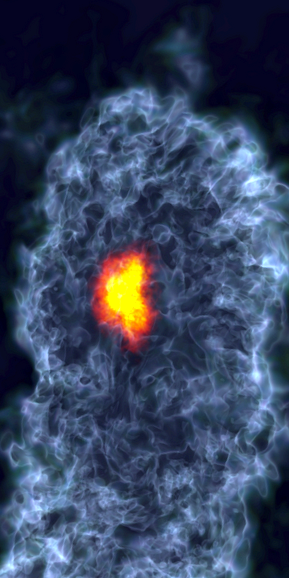
\includegraphics[width=0.875in]{PopIII_vr-edit.png}}
    \centerline{\tiny {[ Sam Skillman, Matt Turk ]}}
\end{minipage}
\end{frame}

  % Why does Enzo-P exist?

%----------------------------------------------------------------------
\NEWSEC \subsection{\ssAmr}
%----------------------------------------------------------------------
\begin{frame}[fragile] 
  \secframetitle{\ssAmr}
  \blockblue
  \begin{block}<+->{\textbf{\enzo\ AMR}}
    \begin{center}
      \begin{minipage}{2.0in}
        \includegraphics<1->[width=2.0in]{enzo-amr.pdf}
      \end{minipage}
    \end{center}
  \end{block}
  \vspace{-0.2in}
  \blockgreen
  \begin{block}<+->{\textbf{\cello\ AMR}}
    \begin{center}
      \begin{minipage}{2.5in}
        \includegraphics<2->[width=2.5in]{cello-amr.pdf}
      \end{minipage}
    \end{center}
  \end{block}
\end{frame}

\begin{frame}[fragile,label=ss-amr] 

  \secframetitle{\ssAmr}
  
  \begin{center}
    \begin{minipage}{1in}
      \includegraphics<1->[width=1in]{enzo-sedov.png}
    \end{minipage} \ 
    \begin{minipage}{2.5in}
      \blockblue
      \begin{block}<+->{\textbf{\enzo}}
        structured AMR \\
        flexibly shaped grids \\
        neighbors \& parent communication \\
        MPI/OpenMP parallel
      \end{block}
    \end{minipage} \\
    \vspace{0.1in}
    \begin{minipage}{1in}
      \includegraphics<2->[width=1in]{cello-sedov.png}
    \end{minipage} \ 
    \begin{minipage}{2.5in}
      \blockgreen
      \begin{block}<+->{\textbf{\enzopcello}}
        array of octrees \\
        fixed shaped blocks \\
        neighbors only communication \\
        Charm++ parallel
      \end{block}
    \end{minipage}
  \end{center}

\end{frame}




%----------------------------------------------------------------------
\NEWSEC \subsection{\ssCharm}
%----------------------------------------------------------------------
%\begin{frame}[fragile,label=ss-charm] 
\secframetitle{\ssCharm}
%--------------------------------------------------
\framesubtitle{MPI parallel programs: passing messages between processes}
%--------------------------------------------------
\begin{minipage}[t]{1.75in}
\begin{center}
\begin{minipage}{1.50in}
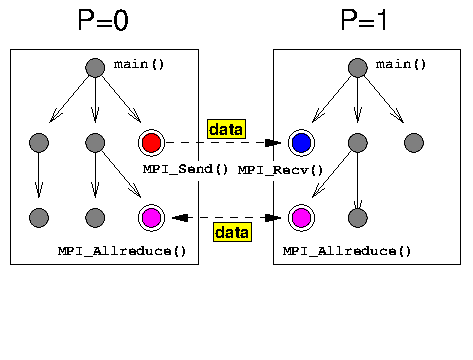
\includegraphics[width=1.50in]{mpi.pdf}\\
\vspace{-0.5in}
\centerline{\scriptsize\textbf{An MPI parallel program}}
\end{minipage}\\ \ \\
%\begin{minipage}{1.25in}
%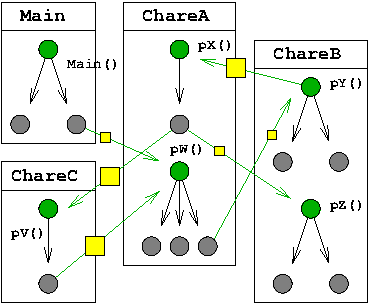
\includegraphics[width=1.25in]{charm.pdf}
%\ \\
%\centerline{\scriptsize\textbf{A Charm\pp\ parallel program}}
%\end{minipage}
\end{center}
\end{minipage} \ 
\begin{minipage}[t]{2.50in}
\vspace{-0.6in}
\begin{itemize}
\item MPI program
  \begin{itemize}
  \item decomposed by \blueit{processes}
  \item calls MPI library
  \item communicate / synchronize
  \end{itemize}
\ \\ \pause
\item MPI runtime system
  \begin{itemize}
  \item sends data between processes
  \item synchronizes between processes
  \end{itemize} \pause
\item Additional features
\begin{itemize}
\item MPI-2: Parallel I/O, remote DMA,
one-sided communication
\item MPI-3: fault-tolerance, hybrid programming, persistence
\end{itemize}
\end{itemize}
\end{minipage}
\end{frame}

\begin{frame}[fragile]
\secframetitle{\ssCharm}
%--------------------------------------------------
\framesubtitle{\charm\ parallel programs: collections of asynchronously-interacting objects}
%--------------------------------------------------
\begin{minipage}[t]{1.75in}
\begin{center}
\begin{minipage}{1.25in}
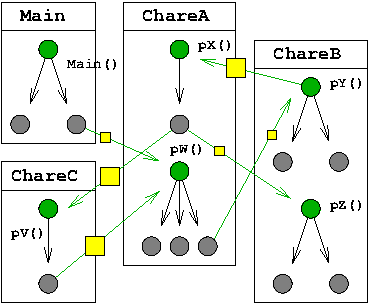
\includegraphics[width=1.25in]{charm.pdf}
\ \\
\centerline{\scriptsize\textbf{A Charm\pp\ parallel program}}
\end{minipage}\\ \ \\
\ \\
\hrule
\ \\
\begin{minipage}{1.50in}
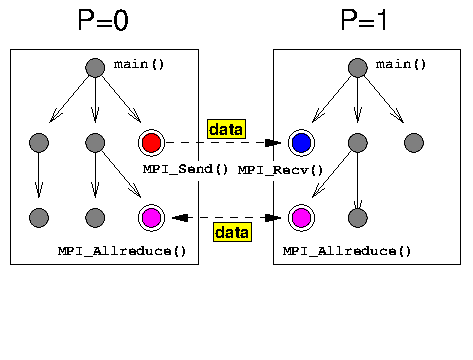
\includegraphics[width=1.50in]{mpi.pdf}\\
\vspace{-0.5in}
\centerline{\scriptsize{An MPI parallel program}}
\end{minipage}
\end{center}
\end{minipage} \ 
\begin{minipage}[t]{2.50in}
\vspace{-0.70in}
\begin{itemize}
\item \charm\ program
  \begin{itemize}
  \item Decomposed by \blueit{objects}
  \item \charm\ objects called \blueit{chares}
  \item invoke \blueit{entry methods}
  \item \blueit{asynchronous}
  \item communicate via \blueit{messages}
  \end{itemize}
\ \\ \pause
\item \charm\ runtime system
  \begin{itemize}
  \item maps chares to processors
  \item schedules entry methods
  \item migrates chares to load balance
  \end{itemize} \pause
\item Additional features
\begin{itemize}
\item checkpoint/restart
\item dynamic load balancing
\item fault-tolerance
\end{itemize}
\end{itemize}
\end{minipage}
\end{frame}

%\begin{frame}[fragile] 
\secframetitle{\ssCharm}
%--------------------------------------------------
%\framesubtitle{Anatomy of a simple Charm program}
%--------------------------------------------------

%     Look at simple HelloWorld Charm++ code
%        Control files
%          *.ci
         
%        Main
%        chare Group
%           one class created per process
% 	  indexed by ip
%        Chare Array
%           at least one class created per process

\begin{itemize}
\item C++ program with ``extra features''
\item Defined using ``\bluecode{.ci}'' control files: 
\begin{itemize}
\item which classes are chares
\item which methods are entry methods
\item declare message objects
\item declare global ``\code{readonly}'' variables
\end{itemize}
\item compiled using \bluecode{charmc}
\item generates \bluecode{.decl.h} and \bluecode{.def.h} from \bluecode{.ci}
\begin{itemize}
\item ``hooks'' program to \charm\ runtime
\item \bluecode{.decl.h} declarations
\item \bluecode{.def.h}: include definitions
\end{itemize}
\item Run executable using \bluecode{charmrun}
\end{itemize}
\end{frame}

%% ----------------------------------------------------------------------
\begin{frame}[fragile] 
\secframetitle{\ssCharm}
\framesubtitle{Chare objects}
\framesubtitle{Chares are concurrent objects}
\begin{itemize}
\item Chares are C++ objects
\item Inherit from \charm\ base class
\footnotesize
\begin{semiverbatim}
#\bluetext{include} \orangetext{"foo.decl.h"}
\bluetext{class} \greentext{Foo} : \bluetext{public} \redtext{CBase_}\greentext{Foo} \{
   \bluetext{Foo} (\greentext{int} \orangetext{n});
   \greentext{void} \bluetext{p_receive_data} (\greentext{int} \orangetext{n}, \greentext{double} * \orangetext{a});
   \greentext{void} \bluetext{print_results} ();
\};
#\bluetext{include} \orangetext{"foo.def.h"}
\end{semiverbatim}
\normalsize
\item Chares and entry methods declared in \code{.ci} control file
\footnotesize
\begin{semiverbatim}
\greentext{module foo} \{
   \greentext{chare} \bluetext{Foo} \{
      \greentext{entry} \bluetext{Foo} (\greentext{int} \orangetext{n});
      \greentext{entry void} \bluetext{p_receive_data} (\greentext{int} \orangetext{n}, \greentext{double} \orangetext{a}[\orangetext{n}]);
   \};
\}
\end{semiverbatim}
\end{itemize}
%\normalsize
%\item \redcode{CBase\_}\greencode{Foo} declared in \bluecode{.decl.h} file
%\item \redcode{CBase\_}\greencode{Foo} defined in \bluecode{.def.h} file
%\end{itemize}
\end{frame}

%% ----------------------------------------------------------------------
\begin{frame}[fragile] 
\secframetitle{\ssCharm}
\framesubtitle{\charm\ control files}

\bluebf{Example control file: \bluecode{hello.ci}}

 \begin{semiverbatim}
    \bluecode{mainmodule} \greencode{hello} \{
       \bluecode{readonly} \greencode{CProxy_Main mainProxy};
       \bluecode{mainchare} \greencode{main} \{
          \bluecode{entry} \greencode{main}(\bluecode{CkArgMsg}*);
       \};
    \};
\end{semiverbatim}
\vspace{-0.2in}
\begin{itemize}
\item \charm\ programs start in a \blueit{mainchare}
\item Other chares created dynamically using \bluecode{ckNew()}
\begin{itemize}
\item new chare may reside remotely
\item \code{ckNew()} returns \blueit{proxy} to chare
\item entry methods called via \bluetext{proxy}
\end{itemize}

\end{itemize}
\end{frame}

%\begin{frame}[fragile] 
\secframetitle{\ssCharm}
\framesubtitle{\charm\ collections of chares}
\vspace{-0.2in}
\begin{center}
\begin{minipage}{4in}
\begin{minipage}{1.5in}
\bluebf{Chare Arrays}
\end{minipage} \ 
\begin{minipage}{2in}

\includegraphics[width=2.0in]{chare-array.pdf}
\end{minipage}
\vspace{0.1in}
  \begin{itemize}
  \item \bluetext{distributed array of chares}
  \item \bluetext{migratable elements}
  \item \bluetext{flexible indexing}
  \end{itemize}
\vspace{0.2in}
\begin{minipage}{1.5in}
\redbf{Chare Groups}
\end{minipage} \ 
\begin{minipage}{2in}
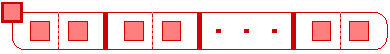
\includegraphics[width=2.0in]{chare-group.pdf}
\end{minipage}
  \begin{itemize}
\setbeamercolor*{item}{fg=red!50!black}
  \item \redtext{one chare per processor (non-migratable)}
  \end{itemize}
\vspace{0.2in}
\begin{minipage}{1.5in}
\greenbf{Chare Nodegroups}
\end{minipage} \ 
\begin{minipage}{2in}
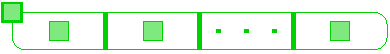
\includegraphics[width=2.0in]{chare-nodegroup.pdf}
\end{minipage}
  \begin{itemize}
\setbeamercolor*{item}{fg=green!50!black}
  \item \greentext{one chare per node (non-migratable)}
  \end{itemize}
\end{minipage}
\end{center}

\end{frame}


%----------------------------------------------------------------------
%======================================================================
\NEWSEC
%======================================================================

\subsection{\ssCompare}

\usebackgroundtemplate
{
\includegraphics[width=5in]{cello-background.png}}
\begin{frame}[fragile,label=ss-compare] 
% ----------------------------------------------------------------------
\secframetitle{\ssCompare}
%\framesubtitle{}
% ----------------------------------------------------------------------
\begin{center}
\rowcolors[]{1}{blue!5}{blue!10}
\begin{tabular}{l|cc} 
 & \textbf{\enzo} & \textbf{\enzopcello} \\ \hline
\uncover<2->{Parallelization} & \uncover<2->{MPI} & \uncover<2->{\charm} \\
\uncover<3->{AMR type}       & \uncover<3->{patch-based} & \uncover<3->{octree-based}   \\
\uncover<4->{AMR structure} & \uncover<4->{replicated} &\uncover<4->{ fully distributed}   \\
\uncover<5->{Time stepping} & \uncover<5->{level-adaptive} & \uncover<5->{block-adaptive$^*$}   \\
\uncover<6->{Block sizes} & \uncover<6->{$\times 1000$ variation} & \uncover<6->{constant}  \\
\uncover<7->{Task scheduling} & \uncover<7->{level-parallel} & \uncover<7->{dependency-driven}  \\
\uncover<8->{Load balancing} & \uncover<8->{patch migration} & \uncover<8->{\charm-based}  \\
\uncover<9->{Data locality} & \uncover<9->{LB conflict} & \uncover<9->{no LB conflict}  \\ 
\uncover<10->{Mesh quality} & \uncover<10->{level jumps} & \uncover<10->{2-to-1 constraint}  \\  \hline
\end{tabular} \\
\uncover<5->{\footnotesize $^*$ not implemented yet}
%  
% \ \\ \ \\
% \url{http://cello-project.org} \\
% NSF PHY-1104819, AST-0808184 \\
% $\qed$
\end{center}
\end{frame}

\usebackgroundtemplate
{}
     % What are the key differences between Enzo-P and Enzo?
%----------------------------------------------------------------------


%----------------------------------------------------------------------
%\NEWSEC \subsection{\ssApproach}
%----------------------------------------------------------------------
%\begin{frame}[fragile,label=ss-approach] 
\secframetitle{\ssApproach}
\framesubtitle{\enzo's limitations}
%\framesubtitle{Scaling issues}
\begin{minipage}{3.0in}
%  AMR data structure scalability
%  Code development and maintenance
%  Ghost zone memory requirement
%  Patch size variation
%  Time stepping
%  Dynamic load balancing
%  Particle positions
%  Mesh quality
% So, how does Cello's AMR try to address the know issues of Enzo's current
% AMR?
%
% The main issues with Enzo's AMR design and implementation involve
% memory usage, the quality of the mesh, parallel task definition
% and scheduling, and data locality.

% [MEMORY] Memory usage is perhaps the most common limitation that
% people run into when running big Enzo simulations.  Enzo's mesh
% hierarchy structure is represented in each MPI process using a
% grid object for each AMR patch.  Although patches assigned to
% remote processors carry no field or particle data, the grid
% objects themselves still take up on the order of a few KB of memory.
% For small hierarchies that's not a problem, but when you have a million
% grid patches that means several GB of memory are required on each
% MPI process.  While supercomputers have gotten larger over the years, the
% amount of memory per node has not---it's still frequently just a few
% GB.  :  Memory fragmentation has also been identified as a problem,
% due to the high volume of heap memory new and delete operations on
% widely varying array sizes.  Ghost zone data can also consume a lot
% of memory, especially for smaller grids.

% [ MESH QUALITY ] Enzo also has known mesh quality issues.  Sometimes
% patches are adjacent to patches in refinement levels that are further than 
% a factor of two different. This can lead to inaccurate interpolation
% compromizing the numerical accuracy of solutions on such patches.

% [ PARALLEL TASKS ] Parallel tasks in Enzo are defined as a grid
% object and its associated field and particle data.  Patch sizes in
% Enzo can vary widly, from large $64^3$ root grid tiles to small
% $8^3$ patches on the finest levels.  Varying task sizes can
% adversely affect performance and load balancing.

\begin{itemize}
\item \bfat{2}{\textcolor{red!50!black}{Memory usage}}
\begin{itemize}
  \item<2-> \textcolor{red}{AMR structure is non-scalable}
  \item<2-> \textcolor{red}{memory fragmentation}
  \item<2-> \textcolor{red}{ghost zones}
\end{itemize}
\item \bfat{3}{\textcolor{green!50!black}{Mesh quality}}
\begin{itemize}
   \item<3-> \textcolor{green!80!black}{2-to-1 refinement constraint violated}
\end{itemize}
\item \bfat{4}{\textcolor{blue!50!black}{Parallel task definition}}
\begin{itemize}
   \item<4-> \textcolor{blue}{widely varying patch sizes}
   \item<4-> \textcolor{blue}{sizes determined by AMR}
\end{itemize}
\item \bfat{5}{\textcolor{cyan!50!black}{Parallel task scheduling}}
\begin{itemize}
   \item<5-> \textcolor{cyan!80!black}{parallel within a level}
   \item<5-> \textcolor{cyan!80!black}{synchronization between level time steps}
\end{itemize}
\item \bfat{6}{\textcolor{orange!50!black}{Data locality}}
\begin{itemize}
   \item<6-> \textcolor{orange!80!black}{disrupted by load balancing}
\end{itemize}
\end{itemize}
\end{minipage} \
\begin{minipage}{1.0in}
\centerline{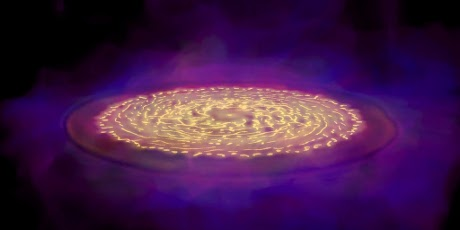
\includegraphics[width=2.0in,angle=90]{iso_and_volume_02_sm.jpg}}
\centerline{\tiny{[ Elizabeth Tasker ]}}
\end{minipage}
\end{frame}

%\begin{frame}[fragile] 
\secframetitle{\ssApproach}
\framesubtitle{\enzopcello\ approach}
%\framesubtitle{Scaling issues}
\begin{minipage}{3.0in}
%  AMR data structure scalability
%  Code development and maintenance
%  Ghost zone memory requirement
%  Patch size variation
%  Time stepping
%  Dynamic load balancing
%  Particle positions
%  Mesh quality
\begin{itemize}
\item \bfat{2}{\textcolor{red!50!black}{Memory usage}}
\begin{itemize}
  \item<2-> \textcolor{red}{AMR structure is fully distributed}
  \item<2-> \textcolor{red}{uniform blocks reduce fragmentation}
  \item<2-> \textcolor{red}{ghost zones allocated when needed$^*$}
\end{itemize}
\item \bfat{3}{\textcolor{green!50!black}{Mesh quality}}
\begin{itemize}
   \item<3-> \textcolor{green!80!black}{2-to-1 refinement constraint maintained}
\end{itemize}
\item \bfat{4}{\textcolor{blue!50!black}{Parallel task definition}}
\begin{itemize}
   \item<4-> \textcolor{blue}{uniform field array sizes in blocks}
   \item<4-> \textcolor{blue}{sizes determined by user}
\end{itemize}
\item \bfat{5}{\textcolor{cyan!50!black}{Parallel task scheduling}}
\begin{itemize}
   \item<5-> \textcolor{cyan!80!black}{asynchronous, data-driven}
   \item<5-> \textcolor{cyan!80!black}{block-local time stepping$^*$}
\end{itemize}
\item \bfat{6}{\textcolor{orange!50!black}{Data locality}}
\begin{itemize}
   \item<6-> \textcolor{orange!80!black}{only nearest-neighbor communication}
\end{itemize}
\end{itemize}
\vspace{-0.1in}
\only<1>{\textcolor{white}{\footnotesize $^*$ not implemented yet}}
\only<2-4>{\textcolor{red}{\footnotesize $^*$ not implemented yet}}
\only<5-6>{\textcolor{cyan!80!black}{\footnotesize $^*$ not implemented yet}}
\end{minipage} \
\begin{minipage}{1.0in}
\vspace{-0.2in}
\centerline{\tiny{Enzo}} 
\vspace{0.1in}
\centerline{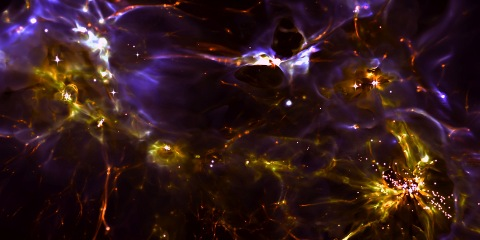
\includegraphics[width=2.0in,angle=90]{jhw-dwarf-galaxies.jpg}}
\centerline{\tiny{[ John Wise ]}}
\end{minipage}
\end{frame}


%----------------------------------------------------------------------
%%======================================================================
\NEWSEC
%======================================================================

\subsection{\ssIntroSummary}

%----------------------------------------------------------------------

\begin{frame}[fragile,label=ss-intro-summary] 
\secframetitle{\ssIntroSummary}

\begin{itemize}
\item Enzo has awesome physics capabilities
\item Enzo also has fast and expertly-crafted numerical methods
\item Main limitations involve underlying data structures
  \begin{itemize}
  \item designed for 1990's supercomputers
  \item hierarchy memory limits scalability
  \item some mesh quality issues
  \end{itemize}
\item \bluetext{Cello} is designed to be a scalable AMR framework
  \begin{itemize}
  \item Charm++ data-driven asynchronous parallelism
  \item scalable forest-of-octree AMR
  \end{itemize}
\item \greentext{Enzo-P} combines Enzo's physics with Cello's AMR
\end{itemize}
\vfill
\centerline{$\qed$}
\end{frame}




%======================================================================
\NEWMOD \section{\sProject}
%======================================================================

%----------------------------------------------------------------------

\logo{\hfill\hyperlink{outline<1>}{\icon}}

\begin{frame}[fragile,label=s-project] 
\modframetitle{\sProject}
\small
\begin{center}
\begin{minipage}{3.25in}
\begin{enumerate}
\item \hyperlink{ss-project<1>}       {\BUTTON {\orow{\ssProject}}} \\
\item \hyperlink{ss-documentation<1>} {\BUTTON {\erow{\ssDocumentation}}} \\
\item \hyperlink{ss-source<1>}        {\BUTTON {\erow{\ssSource}}} \\
%\item \hyperlink{ss-browse<1>}        {\BUTTON {\orow{\ssBrowse}}} \\
\item \hyperlink{ss-bugs<1>}          {\BUTTON {\erow{\ssBugs}}} \\
\item \hyperlink{ss-testing<1>}       {\BUTTON {\orow{\ssTesting}}} \\
%\item \hyperlink{ss-project-summary<1>} {\BUTTON {\erow{\ssProjectSummary}}} \\
%\hyperlink{ss-communicate<1>}   {\BUTTON {\orow{\ssCommunicate}}}
\end{enumerate}
\end{minipage}
\end{center}
\end{frame}

\logo{\hfill\hyperlink{s-project<1>}{\icon}}

%======================================================================
\NEWSEC
%======================================================================

\subsection{\ssProject}

\begin{frame}[fragile,label=ss-project] 
\secframetitle{\ssProject}
\blockblue
\vspace{-0.2in}
\begin{center}
\begin{minipage}{3.5in}
\rowcolors[]{1}{blue!5}{blue!10}
\begin{tabbing}
xxxxx\=xxxxxxxxxxxxxxxxx\= \kill
\rule{\textwidth}{0.1mm} \\[-0.1cm]
\bluetext{\textbf{Project website}} \\[-0.1cm]
 \> \greentext{\url{http://cello-project.org}} \\[-0.2cm]
\rule{\textwidth}{0.1mm} \\[-0.1cm]
\bluetext{{Source code}} \> \> \redtext{\code{cello-src/src}} \\[-0.1cm]
 \> \greentext{\url{https://bitbucket.org/cello-project}} \\[-0.2cm]
\rule{\textwidth}{0.1mm} \\[-0.1cm]
\bluetext{{Documentation}} \>  \> \redtext{\code{cello-doc/source}} \\[-0.1cm]
 \> \greentext{\url{http://cello-project.org/doc}} \\[-0.2cm]
\rule{\textwidth}{0.1mm} \\[-0.1cm]
\bluetext{{Test suite}}  \> \> \redtext{\code{cello-src/test}} \\[-0.1cm]
 \> \greentext{\url{http://cello-project.org/test}} \\[-0.2cm]
\rule{\textwidth}{0.1mm} \\[-0.1cm]
\bluetext{{Bug tracking}} \> \> \redtext{\code{cello-bug}} \\[-0.1cm]
 \> \greentext{\url{http://cello-project.org/bug}}  \\[-0.2cm]
\rule{\textwidth}{0.1mm} \\[-0.1cm]
\bluetext{{Mailing List}} \\[-0.1cm]
 \> \greentext{\footnotesize{\url{https://mailman.ucsd.edu/mailman/listinfo/cello-l/}}}
\end{tabbing}
\end{minipage}
\end{center}

\end{frame}
%----------------------------------------------------------------------
 % How is the Enzo-P project currently organized?
%======================================================================
\NEWSEC
%======================================================================

\subsection{\ssDocumentation}

\begin{frame}[fragile,label=ss-documentation] 
\secframetitle{\ssDocumentation}
\begin{itemize}
\item \greentext{\url{http://cello-project.org} / \framebox{Documentation}}
\begin{itemize}
\item \bluetext{Getting Started Using Enzo-P} \\
      \greentext{download; configure; port; build; run}
\item \bluebf{Enzo-P/Cello parameters reference} \\
      \greenbf{up-to-date list of \textit{all} Enzo-P/Cello parameters}
\item \bluetext{Parameter Files} \\
      \greentext{describes Cello's structured parameter files}
\item \bluetext{Parameter File Example} \\
      \greentext{explains the parameter file used in Getting Started}
\item \bluetext{Enzo-P / Cello Guiding Principles} \\
      \greentext{performance, scalability, usability, reliability, and flexibility}
\item \bluetext{Design} \\
      \greentext{Top-level component design of Cello}
\end{itemize}
\item Documentation is in a state of flux: .pdf $\rightarrow$ .rst
\end{itemize}
\end{frame}

 % What documentation is available?
%======================================================================
\NEWSEC
%======================================================================

\subsection{\ssSource}

\begin{frame}[fragile,label=ss-source] 
\secframetitle{\ssSource}
\begin{itemize}
\item \greentext{\url{https://bitbucket.org/cello-project}}
\item \bluetext{Current project members} \\
\footnotesize
Michael Norman \\
James Bordner \\ 
Tom Abel \\
Greg Bryan \\
Dave Collins \\ 
Alexei Kritsuk \\ 
Brian O'Shea \\
Daniel Reynolds \\ 
Matthew Turk \\ 
John Wise \\
\normalsize
\item \bluetext{Repository:} \redcode{cello-src} \\
\small{\orangecode{hg clone ssh://hg@bitbucket.org/cello-project/cello-src}}
\end{itemize}
\end{frame}

\begin{frame}[fragile] 
\secframetitle{\ssSource}
\begin{itemize}
\item \bluetext{Basic directory structure: \redcode{cello-src/}\ldots} \\
\begin{tabular}{ll}
\redcode{src/Enzo} & \bluetext{Enzo-P source} \\
\redcode{src/Cello} & \bluetext{Cello source} \\
\redcode{bin/enzo-p} & \bluetext{executable} \\
\redcode{input} & \bluetext{sample parameter files} \\
\redcode{test} & \bluetext{tests and results} \\
\redcode{tools} & \bluetext{convenience utilities}
\end{tabular}
\item \bluetext{Some useful files} \\
\begin{tabular}{ll}
\redcode{build.sh} & \bluetext{Build script} \\
\redcode{SContstruct} & \bluetext{Top-level ``make'' file}\\
\redcode{errors.org} & \bluetext{Generated \code{org-mode} errors / warnings} \\
\redcode{diff.org} & \bluetext{Generated \code{org-mode} \greencode{hg diff}} \\
\redcode{log.org} & \bluetext{Generated \code{org-mode} \greencode{hg log}}
\end{tabular}

\end{itemize}
\end{frame}

 % Where is the source code hosted?
%%======================================================================
\NEWSEC
%======================================================================

\subsection{\ssBrowse}

\begin{frame}[fragile,label=ss-browse] 
\secframetitle{\ssBrowse}
\begin{enumerate}
\item \bluetext{Bitbucket}
\begin{itemize}
\item \greentext{\url{https://bitbucket.org/cello-project/cello-src/src}}
\item \bluetext{good for viewing development history}
\end{itemize}
\item \bluetext{Doxygen on \code{cello-project.org} platform}
\begin{itemize}
\item \greentext{\url{http://cello-project.org/src}}
\item \bluetext{good for viewing annotated code structure}
\end{itemize}
\item \bluetext{Doxygen on your laptop}
\begin{itemize}
\item \redcode{make doc}
\item \greentext{\footnotesize\url{file:///home/bordner/Cello/cello-src/}\underline{src-html}\url{/index.html}}
\item \redcode{cd \underline{src-latex}; pdflatex refman.tex}
\end{itemize}
\end{enumerate}

\end{frame}

 % How can I browse the source code?
%======================================================================
\NEWSEC
%======================================================================

\subsection{\ssBugs}

\begin{frame}[fragile,label=ss-bugs] 
\secframetitle{\ssBugs}
\begin{itemize}
\item \greentext{\url{http://cello-project.org} / \framebox{Bug tracking}}
\end{itemize}
\rowcolors[]{1}{blue!5}{blue!10}
\begin{center}
\vspace{-0.1in}
\begin{minipage}{4.5in}
\footnotesize
\begin{tabular}{rll}
% (As of 2015-09-03)
% 2	2013-06-18 	Excessive syncronization during mesh adaptation 
% 3	2013-06-18 	Multiple refresh steps are performed 
% 4	2013-06-18 	ProlongLinear requires ghost depth of four 
% 12	2013-09-10 	Parallel runs may crash in inteuler with numerical errors 
% 13	2014-08-19 	I/O is incorrect for ip stride != 1 
% 19	2015-03-26 	method_ppm-1 and method_ppm-8 produce slightly different results
% 21	2014-03-17 	Small errors near corners of just-refined blocks 
% 31	2014-01-22 	Refresh errors in larger-scale parallel runs 
% 34	2014-02-21 	Several components seem to have memory leaks 
% 36	2014-03-17 	Adapt crashes (surprise) in sdsc-demo.in 
% 40	2014-04-29 	adapt-L5 problem fails sometimes 
% 45	2014-05-11 	Performance output for components seems incorrect 
% 46	2015-05-06 	Adapt seems to not be coarsening some blocks that should coarsen 
% 51	2014-06-27 	Parameter file syntax error messages display incorrect line number 
% 56	2014-08-21 	Restart fails when number of processors is changed 
% 57	2014-09-25 	stale Charm++ array messages in double mach problem cycle 846 
% 59	2014-11-20 	Occasional segmentation faults in file output from dereferencing null file_ pointer 
% 60	2015-07-06 	Load balancing unit tests occasionally hang 
% 68	2015-03-10 	Gravity solver still diverges sometimes 
% 72	2015-05-08 	RefineSlope does not work correctly sometimes 
% 73	2015-06-12 	New implementation of Refresh sometimes hangs sometimes crashes 
% 74	2015-06-16 	Enzo-P crashes in parse.l with Charm version 6.6.1 with P > 1 
% 75	2015-06-18 	method_heat-8 regression test failed 
% 76	2015-07-07 	Refresh add_fields() does not work as expected 
% 78	2015-07-15 	Mg0 solver has grid-effects 
% 79  	2015-07-27      Synchronization in Refresh is incorrect for Mg0
\uncover<1->{ID} & Date & \centerline{\uncover<1->{Summary}} \\
\hline
{\erow{151}} &	2018-05-03 &\erow{Single root block Cosmo crashes in refinement} \\
{\orow{150}} &	2018-04-26 &\orow{Memory leak in Cosmology problems} \\
{\erow{148}} &	2018-04-17 &\erow{load balancing fails when Index bit ordering is changed} \\
{\orow{147}} &	2018-04-17 &\orow{Errors with netlrs smp charm++} \\
{\erow{146}} &	2018-04-02 &\erow{Restart fails for Cosmo\_OsNa problem on SDSC Comet} \\
{\orow{138}} &	2018-02-07 &\orow{Image output fails with ``image\_ already created''} \\
{\erow{126}} &	2017-08-31 &\erow{data output of particles generates corrupt HDF5 files} \\
{\orow{118}} &	2017-07-12 &\orow{HDF5 output does not scale on Blue Waters} \\
{\erow{111}} & 	2017-06-08 &\erow{Adapt fails if octree array axis is not power of 2}
\end{tabular}
\end{minipage}
\end{center}
\end{frame}

 % What are some of the known bugs?
%======================================================================
\NEWSEC
%======================================================================

\subsection{\ssTesting}

\begin{frame}[fragile,label=ss-testing] 
\secframetitle{\ssTesting}
\begin{itemize}
\item \greentext{\url{http://cello-project.org} / \framebox{Regression tests}}
\item \bluetext{Regression tests available in} \redcode{cello-src}
\item \redcode{\$ make test} \bluetext{(takes about 30-60 minutes)}
\item \bluetext{Tests parameter files in} \redcode{cello-src/input}
\item \bluetext{Tests are run in} \redcode{cello-src/test}
\item \bluetext{Test results viewable via}  \redcode{cello-src/test/index.php}
\end{itemize}
\end{frame}

\begin{frame}[fragile] 
\secframetitle{\ssTesting}
\framesubtitle{Enzo-P/Cello Test Results: header table}
\begin{minipage}{1.75in}
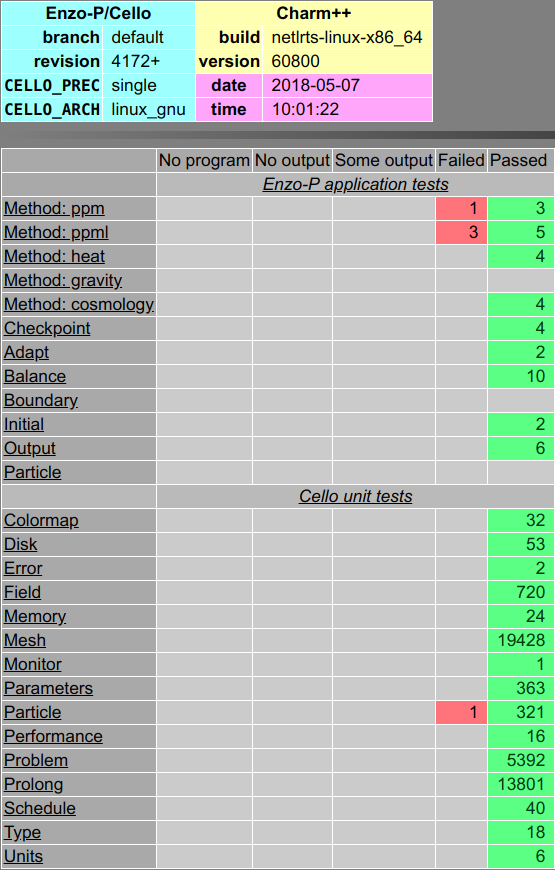
\includegraphics[width=1.75in]{Images/test-1.png}
\end{minipage} \ 
\begin{minipage}{2.25in}
\begin{itemize}
\item Summary of all tests
\item Columns:
\footnotesize
\begin{enumerate}
\item didn't compile
\item didn't start
\item didn't finish
\item tests failed
\item tests passed
\end{enumerate}
\small
\item A few failed tests are expected
\item Sections link to details
\end{itemize}
\end{minipage}
\end{frame}

%----------------------------------------------------------------------

\begin{frame}[fragile] 
\secframetitle{\ssTesting}
\framesubtitle{Enzo-P/Cello Test Results: adaptive mesh refinement}
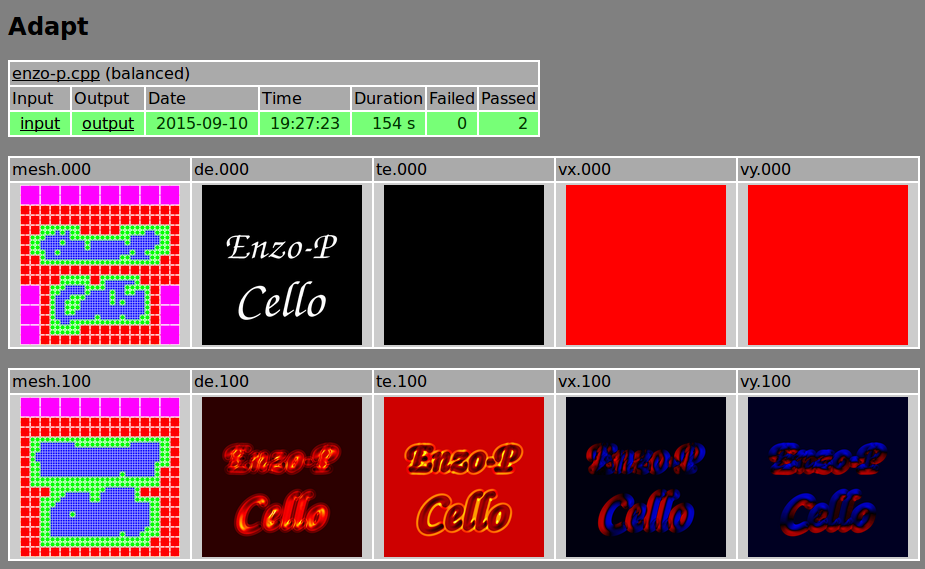
\includegraphics[width=4.0in]{Images/cello-test-2.png}
\end{frame}


\begin{frame}[fragile] 
\secframetitle{\ssTesting}
\framesubtitle{Enzo-P/Cello Test Results: dynamic load balancing}
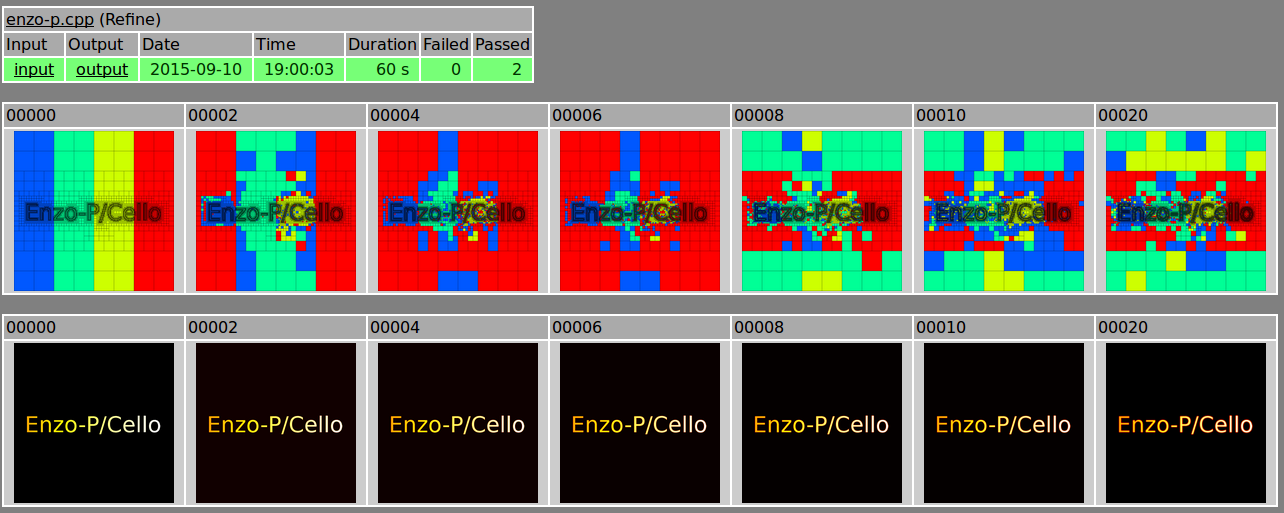
\includegraphics[width=4.0in]{Images/cello-test-3.png}
\end{frame}

 % How is testing done?
%%======================================================================
\NEWSEC
%======================================================================

\subsection{\ssProjectSummary}

%----------------------------------------------------------------------

\begin{frame}[fragile,label=ss-project-summary] 
\secframetitle{\ssProjectSummary}
\begin{itemize}
\item The Enzo-P / Cello project is comprised of multiple components
\item Project page: \url{http://cello-project.org}
\item Source code
\begin{itemize}
\item  \code{http://bitbucket.org/cello-project}
\end{itemize}
\item Documentation
\begin{itemize}
\item doxygen auto-generated:  \code{cello-src/src-html}
\item restructured-text: \code{cello-doc/source}
\end{itemize}
\item Regression testing
\begin{itemize}
\item  \code{cello-src/test}
\item easy to run: \code{make test}
\item results easy to view: \code{cello-src/test/index.php}
\end{itemize}
\item Bug tracking and debugging
\begin{itemize}
\item Bugzilla: \url{http://cello-project.org/bug}
\item Debugging scripts: \code{cello-bug}
\end{itemize}
\end{itemize}
\vfill
\centerline{$\qed$}
\end{frame}

 
%%======================================================================
\NEWSEC
%======================================================================

\subsection{\ssCommunicate}

\begin{frame}[fragile,label=ss-communicate] 
\secframetitle{\ssCommunicate}
\end{frame}

 % How do Enzo-P developers communicate?
  

%======================================================================
\NEWMOD \section{\sPresent}
%======================================================================

%----------------------------------------------------------------------

\logo{\hfill\hyperlink{outline<1>}{\icon}}

\begin{frame}[fragile,label=s-present] 
\modframetitle{\sPresent}
\small
\begin{center}
\begin{minipage}{3.25in}
\begin{enumerate}
\item \hyperlink{ss-state<1>}   {\BUTTON {\ssState}}
%\item \hyperlink{ss-current<1>}   {\BUTTON {\ssCurrent}}
\item \hyperlink{ss-scaling<1>}   {\BUTTON {\ssScaling}}
\item \hyperlink{ss-issues<1>}   {\BUTTON {\ssIssues}}
\item \hyperlink{ss-present-summary<1>}   {\BUTTON {\ssPresentSummary}}
\end{enumerate}
\end{minipage}
\end{center}
\end{frame}

\logo{\hfill\hyperlink{s-present<1>}{\icon}}

%----------------------------------------------------------------------
\NEWSEC \subsection{\ssState}
%----------------------------------------------------------------------

% What is the current state of Enzo-P/Cello?

\begin{frame}[fragile,label=ss-state] 

\secframetitle{\ssState}

%  What is the current state of Enzo-P?  Well, it can do this.

%  This is a pure hydrodynamics problem run using Enzo-P with AMR
%  enabled, with somewhat non-physical initial conditions.

%  It uses an ``array of octrees'' AMR approach, which is simply a
%  uniform array of octrees.  Each Block in the hierarchy contains a
%  small grid of field variables, with size typically around 16^3 to
%  32^3.

%  Enzo-P is parallelized using Charm++ instead of MPI.  Charm++ is an
%  asynchronous data-driven parallel programming language extention to
%  C++.  Each block in the mesh hierarchy is a separate parallel task
%  in Charm, called called a ``chare''.  A key feature of Cello's AMR
%  Charm++ implementation is that it is fully distributed--there is
%  *no* hierarchy meta-data, which addresses a key limitation of
%  the current Enzo.

%  Enzo-P is also designed to be powerful yet easy to use.  While you
%  *can* implement test problem types in Enzo-P like you can Enzo, you
%  can also specify initial and boundary conditions directly in the
%  parameter file.  In this example, initial conditions were generated
%  using a PNG file as a logical mask---the density is initialized to
%  1.5 wherever the PNG file pixels are non-black, otherwise its set
%  to be 12 times less.  This approach means that common test problems
%  such as the implosion problem, Sedov blast wave, or double mach
%  reflection can be set up in the parameter file exclusively without
%  requiring any C++ coding.

\pause
\begin{center}
\begin{minipage}{4.5in}
\begin{minipage}{2.9in}
\only<2->{\vspace{-0.1in}\centerline{in 2014} \ \\ \vspace{-0.2in} \ANIMATEGRAPHICS{width=2.9in}{10}{Images/Daze/daze-0}{000}{100}}
\end{minipage} \ 
\begin{minipage}{1.45in}
\only<3->{\vspace{-0.1in}\centerline{in 2015} \ \\ \vspace{-0.2in}\ANIMATEGRAPHICS{width=1.45in}{10}{Images/1509/1509-0}{00}{56}}
\end{minipage}
\end{minipage}
\end{center}
\pause
\pause
\begin{minipage}[t]{1.2in}
\footnotesize
\vspace{0.1in}
\blockred
\begin{block}<+->{\textbf{Mesh refinement}}
\scriptsize
 \mbox{``array-of-octrees''} \\
 \mbox{field data on blocks} \\ \ \\
\end{block}
\end{minipage} \ \ 
\begin{minipage}[t]{1.0in}
\footnotesize
\vspace{0.1in}
\blockgreen
\begin{block}<+->{\textbf{Parallelism}}
\scriptsize
 Charm++\\
\mbox{blocks are ``chares''} \\
 \mbox{fully-distributed}
\end{block}
\end{minipage} \ \
\begin{minipage}[t]{1.6in}
\raggedright
\footnotesize
\vspace{0.1in}
\blockblue
\begin{block}<+->{\textbf{Parameters}}
\scriptsize
 \mbox{\code{Initial \{ density \{}} \\
 \mbox{\code{ value = [ 1.5, "daze.png",  }} \\
 \mbox{\code{\ \ \ \ \ \ \ \ \ \ \ 0.125 ]; \} \} }}
\end{block}
\end{minipage}

\end{frame}


%----------------------------------------------------------------------

\begin{frame}[fragile,label=ss-state] 
\secframetitle{\ssState}
\begin{center}
\begin{minipage}{4.5in}
\begin{minipage}{2.2in}
\only<2->{\centerline{in 2016}}
\end{minipage}
\begin{minipage}{2.2in}
\only<3->{\centerline{in 2017}}
\end{minipage}
 \vspace{0.2in} \\
\begin{minipage}{2.2in}
\begin{center}
\only<2->{\ANIMATEGRAPHICS{width=1.8in}{10}{Images/Trace/trace-}{00}{99}}
\end{center}
\end{minipage} \
\begin{minipage}{2.2in}
\only<3->{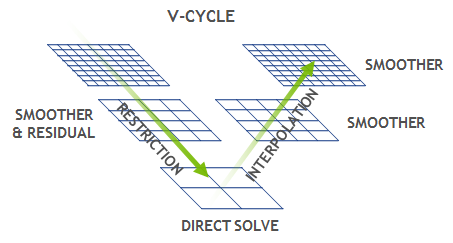
\includegraphics[width=2.0in]{hpgmg_v_cycle.png}}
\end{minipage}
\end{minipage}
\end{center}
\end{frame}


%----------------------------------------------------------------------

\begin{frame}[fragile,label=ss-state] 
\secframetitle{\ssState}
\begin{center}
\centerline{in 2018}  \ \\
\begin{minipage}{4.5in}
\begin{minipage}{2.2in}
\only<1->{\ANIMATEGRAPHICS{width=2.0in}{05}{Images/Comet-run.36/dark-}{00}{21}}
\end{minipage} \
\begin{minipage}{2.2in}
\only<1->{\ANIMATEGRAPHICS{width=2.0in}{05}{Images/Comet-run.36/mesh-}{00}{21}}
\end{minipage}
\end{minipage}
\end{center}
\end{frame}




%======================================================================
\NEWSEC
%======================================================================

% What are Enzo-P's current and near future capabilities?

%\subsection{\ssCurrent}

%% ----------------------------------------------------------------------
\begin{frame}[fragile,label=ss-current] 
\secframetitle{\ssCurrent}

\rowcolors[]{1}{blue!5}{blue!10}
\begin{tabular}{ll}
\uncover<2->{\erow{Physics}} &
\uncover<2->{\erow{PPM, \magentabf{scalable} gravity, (grackle), \magentabf{cosmology}}} \\

\uncover<3->{\orow{Field data}} &
\uncover<3->{\orow{(padding, alignment, precision, centering)}} \\

\uncover<4->{\erow{Particle data}} &
\uncover<4->{\erow{(types, attributes, batches, constants)}} \\

\uncover<5->{\orow{Initial conditions}} &
\uncover<5->{\orow{direct ($f(x,y,z)$), problems (Implosion, Sedov)}} \\

\uncover<6->{\erow{Boundary conditions}} &
\uncover<6->{\erow{inflow ($f(x,y,z,t)$), outflow, reflecting, periodic}} \\

\uncover<7->{\orow{Refinement criteria}} &
\uncover<7->{\orow{slope, density, shear, shock, \magentabf{mass}}} \\

\uncover<8->{\erow{Interpolation}} &
\uncover<8->{\erow{linear, \textcolor{gray}{\enzo's \textit{SecondOrderA}, etc.}}} \\

\uncover<9->{\orow{Time stepping}} &
\uncover<9->{\orow{uniform, \textcolor{gray}{level-adaptive}, \textcolor{gray}{block-adaptive}}} \\

\uncover<10->{\erow{Checkpoint/restart}} &
\uncover<10->{\erow{\charm\ (disk, memory+disk)}} \\

\uncover<11->{\orow{Load balancing}} &
\uncover<11->{\orow{\charm\ (dozens of strategies available)}} \\

\uncover<12->{\erow{I/O}} &
\uncover<12->{\erow{\textcolor{gray}{scalable} HDF5, PNG}} \\
\end{tabular}
\ \\
\ \\
\ \\
\centerline{
\uncover<1->{\magentatext{New capability}} \hfill
\uncover<1->{\bluetext{Pre-existing capability}} \hfill
\uncover<1->{\textcolor{gray}{Not ready yet}}}
\end{frame}


%======================================================================
%\NEWSEC
%======================================================================

% How well does ENzo-P scale?

\subsection{\ssScaling}

%\begin{frame}[fragile,label=ss-scaling] 
\secframetitle{\ssScaling}
\begin{center}
\begin{minipage}{4.50in}
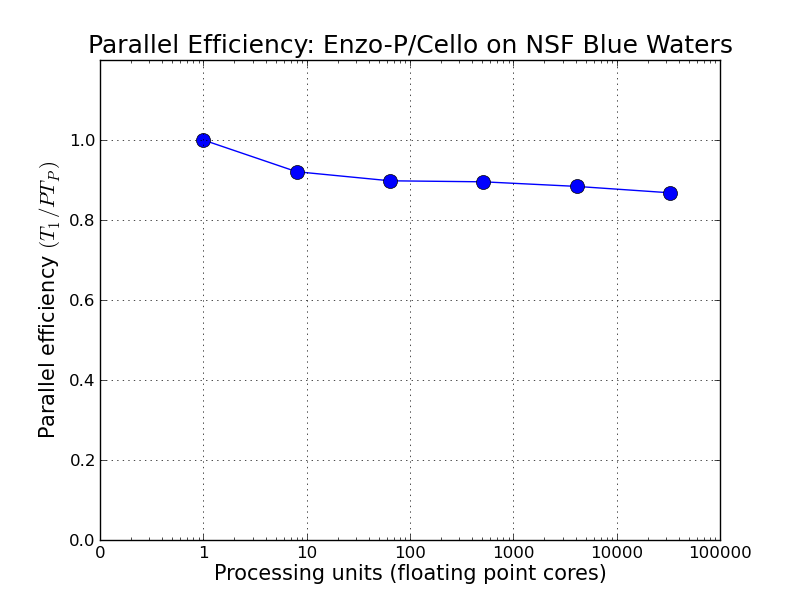
\includegraphics[width=2.25in]{Images/Scaling/scale-eff.png} \ 
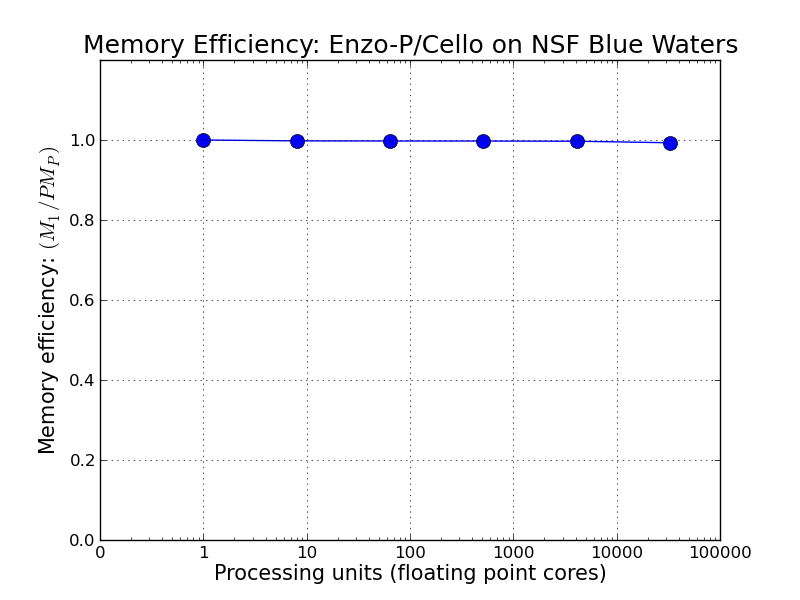
\includegraphics[width=2.25in]{Images/Scaling/scale-mem.png}
\end{minipage} \\
\begin{minipage}{4.0in}
\footnotesize
\pause
\begin{minipage}[t]{1.20in}
\blockblue
\begin{block}<+->{Problem}
%\begin{itemize}
Sedov blast array \\
$L=3$; $32K$ cores \\
$32^3$ cells / block \\
$329$ blocks /core
%\end{itemize}
\end{block}
\end{minipage} \
\begin{minipage}[t]{1.20in}
\blockgreen
\begin{block}<+->{Parallel Efficiency}
%\begin{itemize}
\begin{tabbing}
xxxxxxxxxx\=\kill
Time \> $0.868$ \\
Memory \> $0.993$
\end{tabbing}
%\end{itemize}
\end{block}
\end{minipage} \
\begin{minipage}[t]{1.20in}
\blockred
\begin{block}<+->{Caveats}
%\begin{itemize}
load balanced \\
few refinement steps \\
startup ignored
%\end{itemize}
\end{block}
\end{minipage}
\end{minipage}
\end{center}
\end{frame}

%----------------------------------------------------------------------

\begin{frame}[fragile]
 \secframetitle{\ssScaling}
  \framesubtitle{Hydro and tracer particles: ``Alphabet Soup'' problem}
%   \animategraphics[width=3.5in]{12}{de-2-}{0}{166} 
  \textbf{We tested basic \enzop\ hydrodynamics and particles scalability}
  \begin{minipage}{1.5in}
  \vspace{0.2in}
    \includegraphics<1>[width=1.5in]{Images/Scaling/de-2-3.png} \\
\ \\
    \includegraphics<1>[width=1.5in]{Images/Scaling/age-2-16.png}
  \end{minipage} \
  \begin{minipage}{2.80in}
    \vspace{0.1in}
    \begin{itemize}
    \item variation of ``array of Sedov Blast'' test
    \item letters instead of spheres
      \begin{itemize}
      \item inhibits lockstep coarsen/refine
      \end{itemize}
    \item one ``letter'' per Blue Waters core
    \item tested with/without tracer particles
    \item $32^3$ or $24^3$ cells per block
    \item decent sized AMR problem for 2016
      \begin{itemize}
      \item $256K$ fp-cores
      \item $1.7T$ cells; $0.7T$ (cells + particles)
        \item $50M$ Blocks
      \end{itemize}
      \item \enzo\ would need $72GB$ per process!
    \end{itemize}
    \end{minipage}
\end{frame}


\begin{frame}[fragile]
%--------------------------------------------------  
%--------------------------------------------------  
 \secframetitle{\ssScaling}
  \framesubtitle{Hydro and tracer particles: ``Alphabet Soup'' problem}
%--------------------------------------------------  
\begin{center}
  \vspace{-0.1in}
  \begin{minipage}{4.50in}
    \begin{center}
      \begin{minipage}{2in}
    \includegraphics[width=2.0in]{Images/Scaling/scaling-efficiency-161110.pdf}
    \end{minipage} \ 
      \begin{minipage}{2in}
    \includegraphics[width=2.0in]{Images/Scaling/scaling-time-161110.pdf}
    \end{minipage} \\
    \end{center}
  \end{minipage} \\
\end{center}
\end{frame}


\begin{frame}[fragile]
%--------------------------------------------------  
 \secframetitle{\ssScaling}
\framesubtitle{Hydro, dark matterparticles, gravity: ``Cosmology (non-AMR)'' problem}
%--------------------------------------------------

\textbf{We tested scaling of more recent support for cosmology}

\begin{minipage}{1.5in}
  \vspace{0.2in}
  
\includegraphics[width=1.5in]{Images/Cosmo/dark-20-normal.png} \\
%\centerline{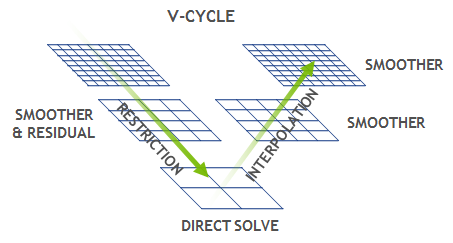
\includegraphics[width=1.5in]{hpgmg_v_cycle.png}}
\end{minipage} \
\begin{minipage}{2.75in}
  \vspace {0.2in}
  \begin{itemize}
  \item PPM hydrodynamics
  \item ``dark matter'' particles
  \item PM gravity method
  \item multigrid solver---non-AMR only
   \item tested up to $128K$ fp-cores
%  \item have since implemented AMR solver
%    \begin{itemize}
%      \item Dan Reynolds ``HG'' algorithm
%    \item preconditioned Krylov solver
%    \item multigrid-based preconditioner
%    \item effective up to $\approx 5$ levels
%    \end{itemize}
  \end{itemize}
\end{minipage}
\end{frame}

\begin{frame}[fragile]
  %--------------------------------------------------  
  \frametitle{\enzopcello\ NSF Blue Waters scaling}
  \framesubtitle{Hydro, particles, gravity: ``Cosmology (non-AMR)'' problem}
  %--------------------------------------------------  
  \begin{center}
    \vspace{-0.1in}
    \begin{minipage}{4.5in}
      \begin{center}
        \begin{minipage}{2.in}
          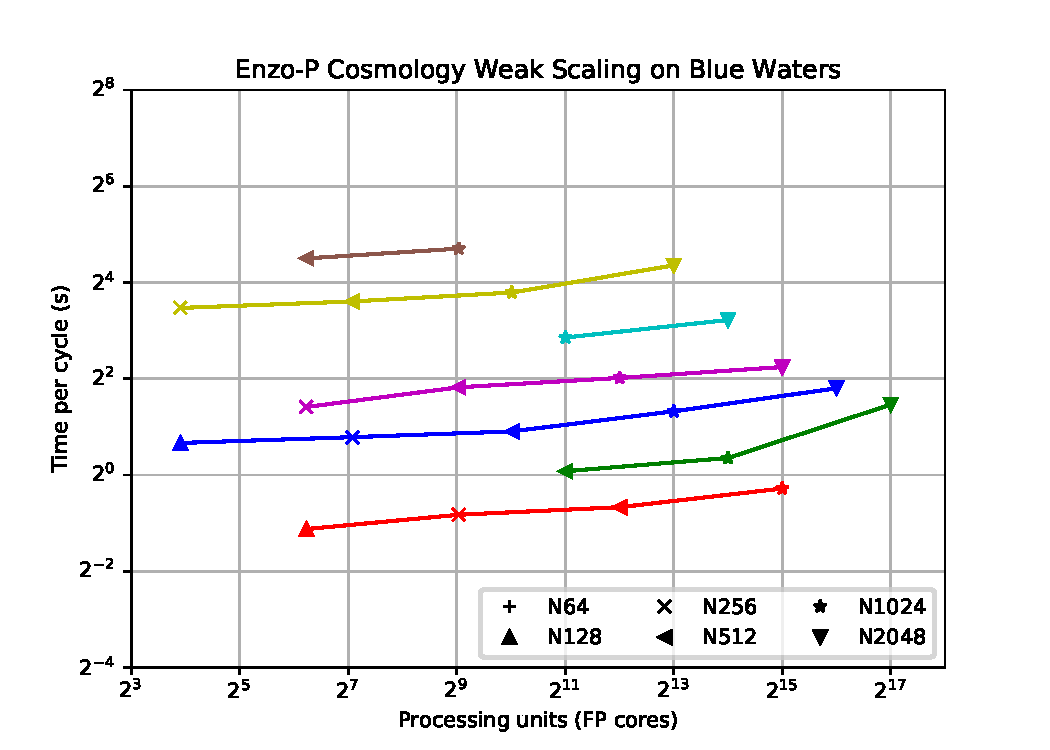
\includegraphics[width=2.2in]{Images/Scaling/smp-cosmo-weak.pdf}
        \end{minipage} \ 
        \begin{minipage}{2.2in}
          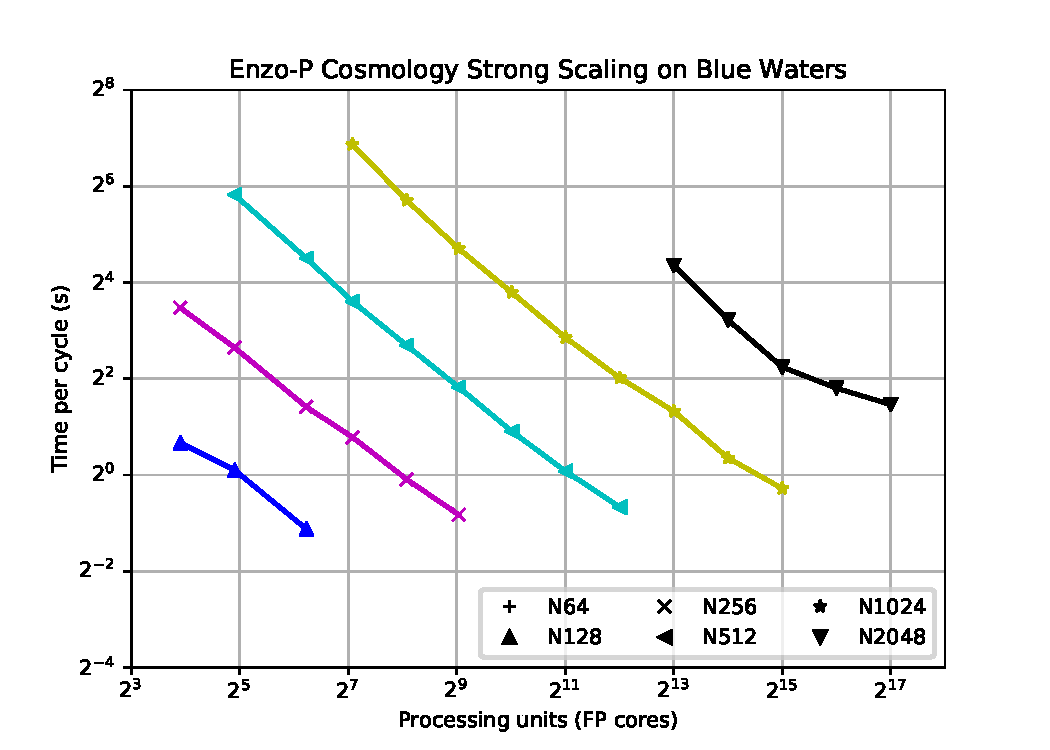
\includegraphics[width=2.2in]{Images/Scaling/smp-cosmo-strong.pdf}
        \end{minipage} \\
      \end{center}
    \end{minipage}
  \end{center}
\end{frame}


%======================================================================
%======================================================================
\NEWSEC
%======================================================================

\subsection{\ssIssues}

\begin{frame}[fragile,label=ss-issues] 
\secframetitle{\ssIssues}
\framesubtitle{Parameter file issues}
% Review ss-bugs.tex / http://client64-249.sdsc.edu/cello-bug

\begin{itemize}
   \item Floats and ints cannot be mixed
   \cornersize{0.9}
   \begin{itemize}
     \item[\frownie] \textcolor{red}{\code{velocity\_x = 8.0 + 2*x }}
     \item[\smiley] \textcolor{green!50!black}{\code{velocity\_x = 8.0 + 2.0*x}}
   \end{itemize}

   \item Need space after subtraction minus sign
   \begin{itemize}
     \item[\frownie] \textcolor{red}{\code{density = x -2.0;}}
     \item[\smiley] \textcolor{green!50!black}{\code{density = x - 2.0;}}
   \end{itemize}
  \item Need at least as many root blocks as processors $P$
  \begin{itemize}
    \item \code{Mesh \{ root\_blocks = [4,4,4]; \} }
    \item[\frownie] \textcolor{red}{\code{\$ charmrun +p72} \code{bin/enzo-p \ldots}}
    \item[\smiley]\textcolor{green!50!black}{\code{\$ charmrun +p64} \code{bin/enzo-p \ldots}}
  \end{itemize}
  \item AMR requires ghost zone depth of $\ge 4$
\end{itemize}

\link{ss-bugs}{Other issues: see bug tracking website}

\end{frame}
      % What are some of Enzo-P's known issues?
%======================================================================

%%======================================================================
\NEWSEC
%======================================================================

\subsection{\ssPresentSummary}

%----------------------------------------------------------------------

\begin{frame}[fragile,label=ss-present-summary] 
\secframetitle{\ssPresentSummary}
\begin{itemize}
\item Enzo-P / Cello now includes gravity as well as hydro
\item (Still only fields, but particles coming very soon)
\item Checkpoint/restart now working
\begin{itemize}
\item ``free'' via \charm
\item checkpoint to file or remote memory
\item automatic fault tolerance possible
\end{itemize}
\item Dynamic load balancing now available
\begin{itemize}
\item ``free'' via \charm
\item dozens of sophisticated schemes available
\end{itemize}
\item Several new refinement criteria implemented
\item Parallel scaling is very promising
\item Codebase could still use some improvement
\end{itemize}
\vfill
\centerline{$\qed$}
\end{frame}



%======================================================================
\NEWMOD \section{\sRecent}
%======================================================================

\logo{\hfill\hyperlink{outline<1>}{\icon}}
\begin{frame}[fragile,label=s-recent] 
\modframetitle{\sRecent}
\small
\begin{center}
\begin{minipage}{3.25in}
\begin{enumerate}
\item \hyperlink{ss-recent-solvers<1>}   {\BUTTON {\ssRecentSolvers}}
\item \hyperlink{ss-recent-music<1>}      {\BUTTON {\ssRecentMusic}}
\item \hyperlink{ss-recent-scalable-gravity<1>}   {\BUTTON {\ssRecentScalableGravity}}
\item \hyperlink{ss-recent-expansion<1>}   {\BUTTON {\ssRecentExpansion}}
\item \hyperlink{ss-recent-cosmology<1>}   {\BUTTON {\ssRecentCosmology}}
\item \hyperlink{ss-recent-ppm-devel<1>}   {\BUTTON {\ssRecentPpmDevel}}
\item \hyperlink{ss-recent-misc<1>}   {\BUTTON {\ssRecentMisc}}
%@@@@@@@@@@@@@@@@
%\item \hyperlink{ss-recent-particles<1>}   {\BUTTON {\ssRecentParticles}}
%\item \hyperlink{ss-recent-gravity<1>}     {\BUTTON {\ssRecentGravity}}
%\item \hyperlink{ss-recent-history<1>}     {\BUTTON {\ssRecentHistory}}
%\item \hyperlink{ss-recent-temporary<1>}     {\BUTTON {\ssRecentTemporary}}
\end{enumerate}
\end{minipage}
\end{center}
\end{frame}

\logo{\hfill\hyperlink{s-recent<1>}{\icon}}

%======================================================================
\NEWSEC
%======================================================================


\subsection{\ssRecentGravity}



%----------------------------------------------------------------------
%  Scalable AMR Solvers
%  
%
\begin{frame}[fragile,label=ss-recent-solvers] 
  \secframetitle{\ssRecentSolvers}
  \begin{itemize}
  \item Previously had individual \verb+"EnzoMethodGravity+\textit{<solver>}\verb+"+ \code{Methods}
\begin{verbatim}
   Method {
      list = [ ... "gravity_bicgstab" ... ];
      gravity_bicgstab {
         max_iter = 1000;
         res_tol  = 0.01;
      }
   }
\end{verbatim}
    \vspace{-0.1in}
  \item Now have single \code{EnzoMethodGravity} \code{Method}
  \item Now have separate \code{Solver} classes for linear solvers
  \begin{itemize}
    \item \code{EnzoSolverCg}: Conjugate gradient method (symmetric only)
    \item \code{EnzoSolverBiCgStab}: stabilized Bi-conjugate gradient
    \item \code{EnzoSolverMg0}: Multigrid V-cycle solver (unigrid only)
  \end{itemize}
    \end{itemize}
\end{frame}

%----------------------------------------------------------------------

\begin{frame}[fragile,label=ss-recent-solvers] 
  \secframetitle{\ssRecentSolvers}
  \begin{itemize}
  \item Specify solver with \verb+solver+ paramater
    \small
\begin{verbatim}
   Method {
      list = [ ... "gravity" ... ];
      gravity {
         solver = "bcg";
      }
   }
   Solver {
      list = ["bcg"];
      bcg {
         type = "bicgstab";
         max_iter = 1000;
         res_tol  = 0.01;
      }
   }
\end{verbatim}
%        Used to be different 
%          for each solver.
%        solver code couldn't be reused for non-gravity
%        duplicate gravity-related code
%  
%        Old parameters
%
%       New parameters
%#+BEGIN_SRC text
    %#+END_SRC
    \end{itemize}
\end{frame}
%
 % have Solvers objects
%======================================================================
\NEWSEC
%======================================================================


\subsection{\ssRecentMusic}




%----------------------------------------------------------------------
%  MUSIC initial conditions
%  
%
\begin{frame}[fragile,label=ss-recent-music] 
  \secframetitle{\ssRecentMusic}
  \begin{itemize}
  \item Can read in MUSIC initial conditions: \code{EnzoInitialMusic}
  \item Support both field data and particle data
\small
\begin{verbatim}
   Initial {
      list = [ ... "music" ... ];
      music {
         file_list = [ "FD", ... , "PX", ... ];
         FD {
            type = "field";
            ...
         }
         PX {
            type = "particle";
            ...
         }
      }
   }
\end{verbatim}
\end{itemize}
\end{frame}

\begin{frame}[fragile,label=ss-recent-music] 
  \secframetitle{\ssRecentMusic}
  \begin{itemize}
  \item Field file parameters
    \small
  \begin{verbatim}
   FD {
      name = "density";
      file = "GridDensity";
      dataset = "GridDensity";
      coords = "tzyx";
   }
         \end{verbatim}
  \item Particle file parameters
    \small
  \begin{verbatim}
   PX {
      name = "dark";
      attribute = "x";
      file = "ParticleDisplacements_x";
      dataset = "ParticleDisplacements_x";
      coords = "tzyx";
   }
   \end{verbatim}
\end{itemize}
\end{frame}

    %           MUSIC Input data files
%           EnzoInitialMusic class
%           supports both particles and fields
%           Currently unigrid only
%           Each Block figures out what section to read
%           AMR should be relatively painless
%   
% #+BEGIN_SRC text
%       }
%      }
% #+END_SRC

  %
 % MUSIC initial conditions
%======================================================================
\NEWSEC
%======================================================================


\subsection{\ssRecentScalableGravity}

\begin{frame}[fragile,label=ss-recent-scalable-gravity] 
\secframetitle{\ssRecentScalableGravity}

\begin{itemize}
%   - [ ] create performance plots / movies
  \item New solver: ``HG'' algorithm
  \begin{itemize}
    \item developed by Dan Reynolds
    \item designed for modest refinement levels
%    \item No separate \code{EnzoSolverHg} class
    \item implemented as preconditioned BiCgStab
    \begin{itemize}
      \item Mg0 V-cycle preconditioner
      \item no smoothings going up/down hierarchy
      \item final Jacobi smoothing
    \end{itemize}
    \item restart with previous solution
  \end{itemize}
  \item Additional gravity improvements
  \begin{itemize}
    \item corrected ghost refresh (accumulate for particle mass)
    \item higher level discretizations in \code{EnzoMatrixLaplacian}
    \item incorporate \verb+dep_grid_cic()+ for centered-time gas
  \end{itemize}
\end{itemize}
\end{frame}

 % scalable gravity solvers
%======================================================================
\NEWSEC
%======================================================================

\subsection{\ssRecentExpansion}

\begin{frame}[fragile,label=ss-recent-expansion] 
\secframetitle{\ssRecentExpansion}
\begin{itemize}
\item Britton implemented comoving expansion
\item \code{EnzoMethodComovingExpansion} calls \verb+expand_terms()+
\item Cosmology initial conditions
\begin{itemize}
\item \code{EnzoInitialMusic}: read MUSIC I.C.'s
\item \code{EnzoInitialCosmology}: compute energies, initial redshift
\begin{verbatim}
  Initial {
    list = [ "music", "cosmology" ];
    ...
  }
\end{verbatim}
\end{itemize}
\item Incorporate expansion factors in \code{EnzoComputeAcceleration}
\item \code{EnzoUnits : public Units} supports expansion factors
\end{itemize}
\end{frame}


% \begin{frame}[fragile,label=ss-recent-cosmology] 
% \secframetitle{\ssRecentCosmology}
% Cosmological parameters are set in the \code{Physics} parameter group.
% \small
% \begin{tabbing}
% \code{xxx}\=\code{xxx}\=\code{xxx}\=\code{xxxxxxxxxxxxxxxxxxxxx}\=\kill
% \>\code{Physics \{ } \\
% \> \> \code{list = ["cosmology"];} \\
% \> \> \code{cosmology \{ } \\
% \>\>\> \code{hubble\_constant\_now} \> \code { = 0.701; } \\
% \>\>\> \code{omega\_matter\_now} \> \code{ =   0.279; } \\
% \>\>\> \code{omega\_dark\_matter\_now} \> \code { =   -1.0; } \\
% \>\>\> \code{omega\_lambda\_now} \> \code { =   0.721; } \\
% \>\>\> \code{comoving\_box\_size} \> \code { = 64.0; } \\
% \>\>\> \code{max\_expansion\_rate} \> \code { = 0.01; } \\
% \>\>\> \code{initial\_redshift} \> \code { =  20.0; } \\
% \>\>\> \code{final\_redshift} \> \code { =  0.0; } \\
% \>\>  \code{ \} } \\
% \>  \code{ \} }
% \end{tabbing}
% \end{frame}

% ----------------------------------------------------------------------


% \begin{frame}[fragile]
% \secframetitle{\ssRecentCosmology}
% Cosmological parameters are stored in an \code{EnzoPhysicsCosmology} object.
% \footnotesize
% \begin{tabbing}
% \code{xxx}\=\code{xxx}\=\code{xxxxxxxxxxxxxxxxxxx}\=\kill
% \> \code{EnzoPhysicsCosmology * cosmology = (EnzoPhysicsCosmology * )} \\
% \> \> \code{      simulation()->problem()->physics("cosmology");} \\
% \\ 
% \> \code{enzo\_float omega\_lambda\_now =} \\
% \>\> \code{cosmology->omega\_lambda\_now()} \\
% \> \code{enzo\_float time\_begin =} \\
% \>\> \code{cosmology->initial\_time\_in\_code\_units();} \\
% \\
% \> \code{cosmology->compute\_expansion\_factor (\&a,\&dadt, time);} \\
% \> \code{cosmology->compute\_expansion\_timestep (\&dt\_expansion, time);} \\ 
% \> \code{cosmology->get\_units (\&density\_units,} \\
% \>\>\> \code{\&length\_units,} \\
% \>\>\> \code{\&temperature\_units,} \\
% \>\>\> \code{\&time\_units,} \\
% \>\>\> \code{\&velocity\_units,} \\
% \>\>\> \code{time);}
% \end{tabbing}
% \end{frame}

 % have cosmological expansion
%======================================================================
\NEWSEC
%======================================================================

\subsection{\ssRecentCosmology}

\begin{frame}[fragile,label=ss-recent-cosmology] 
\secframetitle{\ssRecentCosmology}
\begin{itemize}
\item Block size $32^3$
\end{itemize}
\begin{center}
\begin{minipage}{2.0in}
\only<1->{\ANIMATEGRAPHICS{width=2.0in}{05}{Images/Comet-run.34/dark-}{00}{33}}
\end{minipage} \ 
\begin{minipage}{2.0in}
\only<1->{\ANIMATEGRAPHICS{width=2.0in}{05}{Images/Comet-run.34/mesh-}{00}{33}}
\end{minipage}
\end{center}
\end{frame}

%----------------------------------------------------------------------

\begin{frame}[fragile,label=ss-recent-cosmology] 
\secframetitle{\ssRecentCosmology}
\begin{itemize}
\item Block size $16^3$
\end{itemize}
\begin{center}
\begin{minipage}{2.0in}
\only<1->{\ANIMATEGRAPHICS{width=2.0in}{05}{Images/Comet-run.35/dark-}{00}{26}}
\end{minipage} \ 
\begin{minipage}{2.0in}
\only<1->{\ANIMATEGRAPHICS{width=2.0in}{05}{Images/Comet-run.35/mesh-}{00}{26}}
\end{minipage}
\end{center}
\end{frame}

%----------------------------------------------------------------------


\begin{frame}[fragile,label=ss-recent-cosmology] 
\secframetitle{\ssRecentCosmology}
\begin{itemize}
\item Block size $8^3$
\end{itemize}
\begin{center}
\begin{minipage}{2.0in}
\only<1->{\ANIMATEGRAPHICS{width=2.0in}{05}{Images/Comet-run.36/dark-}{00}{21}}
\end{minipage} \ 
\begin{minipage}{2.0in}
\only<1->{\ANIMATEGRAPHICS{width=2.0in}{05}{Images/Comet-run.36/mesh-}{00}{21}}
\end{minipage}
\end{center}
\end{frame}


\begin{frame}[fragile,label=ss-recent-cosmology] 
\secframetitle{\ssRecentCosmology}
\centerline{Block size $32^3$ runs the fastest}
\begin{center}
\begin{minipage}{3.5in}
\only<1->{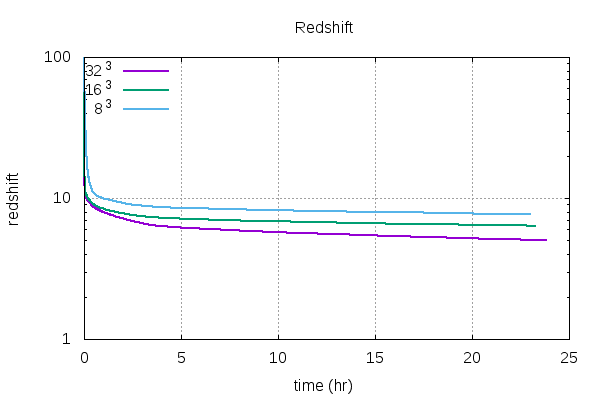
\includegraphics[width=3.5in]{Images/b345-redshift.png}}
\end{minipage} \ 
\end{center}
\end{frame}

\begin{frame}[fragile,label=ss-recent-cosmology] 
\secframetitle{\ssRecentCosmology}
\centerline{But block size $32^3$ uses the most memory}
\begin{center}
\begin{minipage}{3.5in}
\only<1->{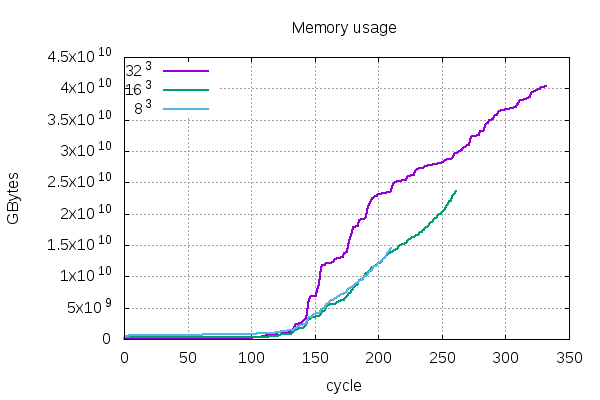
\includegraphics[width=3.5in]{Images/b345-bytes.png}}
\end{minipage} \ 
\end{center}
\end{frame}

\begin{frame}[fragile,label=ss-recent-cosmology] 
\secframetitle{\ssRecentCosmology}
\centerline{Time per cycle has a burst of growth at varying points}
\begin{center}
\begin{minipage}{3.5in}
\only<1->{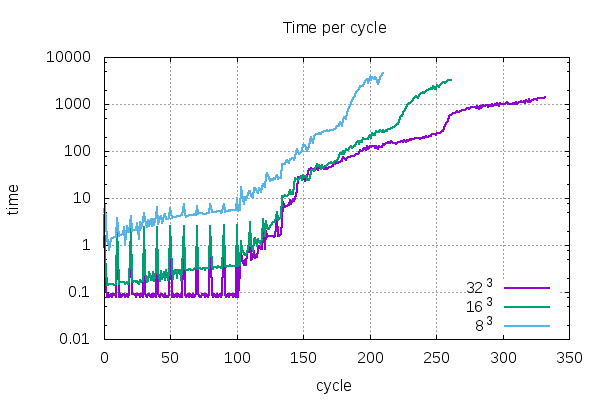
\includegraphics[width=3.5in]{Images/b345-time-per-cycle-log.png}}
\end{minipage}
\end{center}
\end{frame}

\begin{frame}[fragile,label=ss-recent-cosmology] 
\secframetitle{\ssRecentCosmology}
\centerline{Solver time scaled by number of blocks shows this even more}
\begin{center}
\begin{minipage}{3.5in}
\only<1->{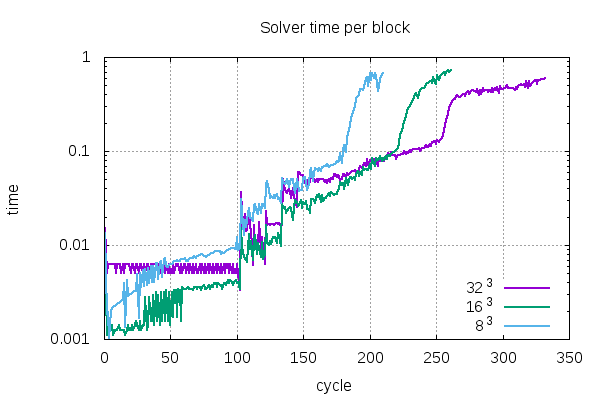
\includegraphics[width=3.5in]{Images/b345-time-per-block.png}}
\end{minipage}
\end{center}
\end{frame}

\begin{frame}[fragile,label=ss-recent-cosmology] 
\secframetitle{\ssRecentCosmology}
\centerline{Yet number of solver iterations is very reasonable}
\begin{center}
\begin{minipage}{3.5in}
\only<1->{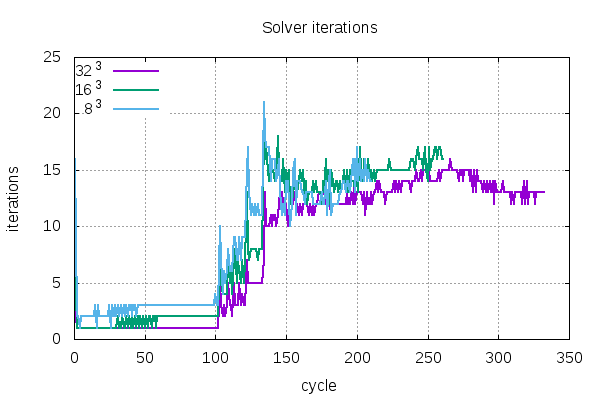
\includegraphics[width=3.5in]{Images/b345-bcg-iters.png}}
\end{minipage}
\end{center}
\end{frame}

\begin{frame}[fragile,label=ss-recent-cosmology] 
\secframetitle{\ssRecentCosmology}
\centerline{Memory per block is also increasing}
\begin{center}
\begin{minipage}{3.5in}
\only<1->{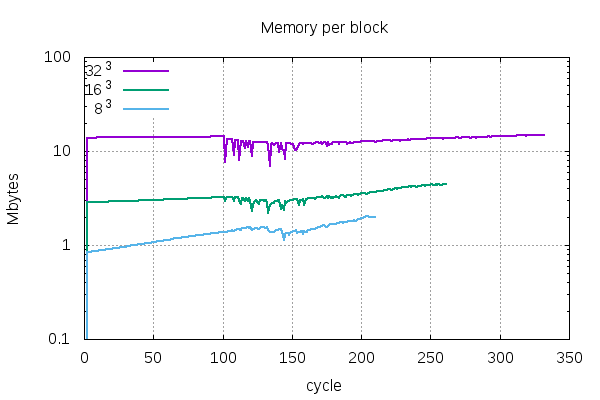
\includegraphics[width=3.5in]{Images/b345-bytes-per-block.png}}
\end{minipage}
\end{center}
\end{frame}

% \begin{frame}[fragile,label=ss-recent-cosmology] 
% \secframetitle{\ssRecentCosmology}
% Cosmological parameters are set in the \code{Physics} parameter group.
% \small
% \begin{tabbing}
% \code{xxx}\=\code{xxx}\=\code{xxx}\=\code{xxxxxxxxxxxxxxxxxxxxx}\=\kill
% \>\code{Physics \{ } \\
% \> \> \code{list = ["cosmology"];} \\
% \> \> \code{cosmology \{ } \\
% \>\>\> \code{hubble\_constant\_now} \> \code { = 0.701; } \\
% \>\>\> \code{omega\_matter\_now} \> \code{ =   0.279; } \\
% \>\>\> \code{omega\_dark\_matter\_now} \> \code { =   -1.0; } \\
% \>\>\> \code{omega\_lambda\_now} \> \code { =   0.721; } \\
% \>\>\> \code{comoving\_box\_size} \> \code { = 64.0; } \\
% \>\>\> \code{max\_expansion\_rate} \> \code { = 0.01; } \\
% \>\>\> \code{initial\_redshift} \> \code { =  20.0; } \\
% \>\>\> \code{final\_redshift} \> \code { =  0.0; } \\
% \>\>  \code{ \} } \\
% \>  \code{ \} }
% \end{tabbing}
% \end{frame}

% ----------------------------------------------------------------------


% \begin{frame}[fragile]
% \secframetitle{\ssRecentCosmology}
% Cosmological parameters are stored in an \code{EnzoPhysicsCosmology} object.
% \footnotesize
% \begin{tabbing}
% \code{xxx}\=\code{xxx}\=\code{xxxxxxxxxxxxxxxxxxx}\=\kill
% \> \code{EnzoPhysicsCosmology * cosmology = (EnzoPhysicsCosmology * )} \\
% \> \> \code{      simulation()->problem()->physics("cosmology");} \\
% \\ 
% \> \code{enzo\_float omega\_lambda\_now =} \\
% \>\> \code{cosmology->omega\_lambda\_now()} \\
% \> \code{enzo\_float time\_begin =} \\
% \>\> \code{cosmology->initial\_time\_in\_code\_units();} \\
% \\
% \> \code{cosmology->compute\_expansion\_factor (\&a,\&dadt, time);} \\
% \> \code{cosmology->compute\_expansion\_timestep (\&dt\_expansion, time);} \\ 
% \> \code{cosmology->get\_units (\&density\_units,} \\
% \>\>\> \code{\&length\_units,} \\
% \>\>\> \code{\&temperature\_units,} \\
% \>\>\> \code{\&time\_units,} \\
% \>\>\> \code{\&velocity\_units,} \\
% \>\>\> \code{time);}
% \end{tabbing}
% \end{frame}

 % have scalable AMR cosmology
%======================================================================
\NEWSEC
%======================================================================



\subsection{\ssRecentPpmDevel}

\begin{frame}[fragile,label=ss-recent-ppm-devel] 
\secframetitle{\ssRecentPpmDevel}
\begin{itemize}
\item PPM hydrodynamics updated from enzo-dev ``week-of-code''
\item old PPM still available: in \code{SContruct} set \code{new\_ppm=0}
\item new changes to ENZO PPM can be tracked using \code{diff}:
\footnotesize
\begin{verbatim}
    diff -bB calcdiss_dev.F ~/Enzo/enzo-dev/src/enzo/calcdiss.F 
    1,2c1
    < #include "fortran.h"
    < #define FORTRAN
    ---
    > #include "fortran.def"
    18c17
    <       subroutine calcdiss_dev(
    ---
    >       subroutine calcdiss(
    115c114
    < #include "fortran_types.h"
    ---
    > #include "fortran_types.def"
\end{verbatim}
\end{itemize}

\end{frame}

 % Updated PPM devel
%======================================================================
\NEWSEC
%======================================================================


\subsection{\ssRecentMisc}

\begin{frame}[fragile,label=ss-recent-misc] 
\secframetitle{\ssRecentMisc}
\begin{itemize}
\item \code{Yt} interface for Enzo-P (Britton Smith)
\begin{itemize}
\item may need trivial tweak to work
\item (``\verb+particle dark+'' -> ``\verb+particle_dark+'')
\item uses \verb+parameters.libconfig+ file of Enzo-P parameters
\item Enzo-P parameter names are subject to change
\end{itemize}
\item \verb+sedov_random+ problem initialier (Thomas Bolden)
\item \code{RefineByMass} has been updated
\begin{itemize}
\item \verb+"dark"+ and \verb+"baryon"+ supported individually
\item includes updates for cosmology
\end{itemize}
\item Updating some things to C++-11/C++-14
\begin{itemize}
\item  smart pointers
\item  auto variables
\end{itemize}
\end{itemize}
\end{frame}
 % Miscellaneous

%@@@@@@@@@@@@@@@@@
%%======================================================================
\NEWSEC
%======================================================================

\subsection{\ssRecentParticles}

%----------------------------------------------------------------------
\begin{frame}[fragile,label=ss-recent-particles] 
  \secframetitle{\ssRecentParticles}
  \framesubtitle{Cello supports Particles!}

\begin{minipage}{2.5in}
\begin{itemize}
\item user-defined types
\begin{itemize}
        \item  declared in input parameter file
        \item  \bluecode{"trace"}: tracer particles
        \item  \bluecode{"dark"}: dark matter particles
        \item  others defined as needed
\end{itemize}
\item each with own list of attributes
\begin{itemize}
        \item  position (\bluecode{"x"},\bluecode{"y"},\bluecode{"z"})
        \item  velocity (\bluecode{"vx"},\bluecode{"vy"},\bluecode{"vz"})
        \item  mass (\bluecode{"mass"})
        \item  id (\bluecode{"id"})
        \item \textit{integer} (8-,16-,32-,64-bit)
        \item \textit{float}   (32-, 64-, 128-bit)
        \end{itemize}
\item constant attributes available
\end{itemize}
\end{minipage} \
\begin{minipage}{2.0in}
%\ANIMATEGRAPHICS{width=1.25in}{20}{Images/Trace/Trace-0}{000}{010}
\end{minipage}
\end{frame}

%======================================================================

\begin{frame}[fragile,label=ss-recent-particles] 
  \secframetitle{\ssRecentParticles}
\framesubtitle{How \code{Particle} objects store particle data}
\begin{minipage}{1.8in}
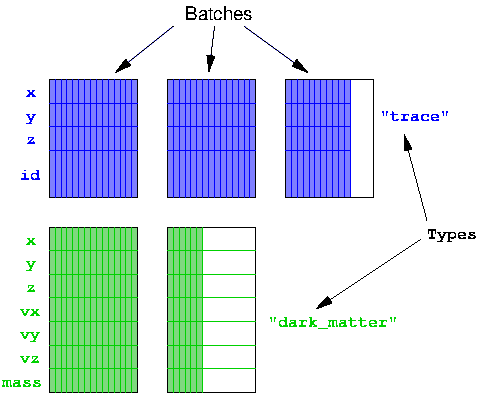
\includegraphics[width=2.0in]{particles-design.pdf} \ \\
\end{minipage} \ 
\begin{minipage}{2.5in}
\begin{itemize}
\item multiple particle \textit{types}
\item particles allocated in \textit{batches}
\begin{itemize}
\item fixed size arrays
\item fewer new/delete operations
\item efficient insert/delete operations
\item potentially useful for GPU's
\end{itemize}
\item batches store particle \textit{attributes}
\begin{itemize}
\item (position, velocity, mass, etc.)
\item 8,16,32,64-bit integers
\item 32,64,128-bit floats
\end{itemize}
\end{itemize}
\end{minipage}
\begin{itemize}
\item particle positions may be floating-point or integers
\begin{itemize}
\item floating-point for storing global positions
\item integers for \code{Block}-local coordinates
\begin{itemize}
\item solves reduced precision issue for deep hierarchies
\item less memory required for given accuracy
\end{itemize}
\end{itemize}
\end{itemize}
\end{frame}

%----------------------------------------------------------------------
%
% Review of Particles in Cello
%
%   Particles that move between blocks are handled by Cello
%
%   Cello handles moving particles
%     4^3 array
%     one-pass through particles to sort and scatter
%     particles
%

\begin{frame}[fragile,label=ss-recent-particles] 
  \secframetitle{\ssRecentParticles}
  \framesubtitle{Particle communication between Blocks}
\begin{itemize}
\item communication is required when particles move outside a Block 
\item this is done using a 4x4x4 array
\begin{itemize}
\item array contains pointers to ParticleData (PD) objects
\item one PD object per neighbor Block
\end{itemize}

\end{itemize}
\begin{minipage}{1.8in}
%\includegraphics<1>[width=2.0in]{particle-refresh-0.pdf}
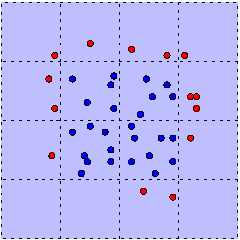
\includegraphics[width=2.0in]{particle-refresh-2.pdf}
%\includegraphics<4>[width=2.0in]{particle-refresh-3.pdf}
%\includegraphics[width=2.0in]{particle-refresh-4.pdf}
\end{minipage} \ 
\begin{minipage}{2.7in}
\begin{itemize}
\item migrating particles are
\begin{itemize}
\item \code{scatter()}-ed to PD array objects
\item sent to associated neighbors
\item \code{gather()}-ed by neighbors
\end{itemize}
\item one sweep through particles
\item one communication step per neighbor
%\item similar for refinement / coarsening
\end{itemize}
\end{minipage}
\end{frame}

%----------------------------------------------------------------------
%  
%   Class structure of particles in Cello mirrors Field classes
%
%   Particle: particles as seen by application
%     ParticleDescr: ``descriptor'' class defining particle parameters
%     ParticleData: ``data'' class containing block particle data
%

%\begin{frame}[fragile,label=ss-recent-particles] 
%  \secframetitle{\ssRecentParticles}
%  \framesubtitle{Class structure of particles}
%
%\end{frame}

%----------------------------------------------------------------------

\begin{frame}[fragile,label=ss-recent-particles] 
  \secframetitle{\ssRecentParticles}
  \framesubtitle{Particle type parameters}
Particles are declared in the input parameter file using the Particle group

\begin{tabbing}
\code{xxxxxx}\=\code{xxxxx}\=\code{xxxxxxxxxxxxxx}\=\kill
\code{Particle \{} \\
\>    \code{list = ["trace"];} \\
\\
\>    \code{trace \{} \\
\> \>     \code{attributes = ["id", "int64",} \\
\> \> \> \code{\ "x", "single",} \\
\> \> \> \code{\ "y", "single",} \\
\> \> \> \code{\ "z", "single"];} \\
\> \>      \code{position = ["x","y","z"];} \\
\> \>      \code{batch\_size = 2000; } \\
\>    \code{\} } \\
\code{\} }
\end{tabbing}
\end{frame}

%----------------------------------------------------------------------

\begin{frame}[fragile,label=ss-recent-particles] 
  \secframetitle{\ssRecentParticles}
  \framesubtitle{Particle type parameters}
  \small
\begin{tabbing}
\code{xx}\=\code{xx}\=\code{xxx}\=\kill
\code{Particle \{} \\
\>    \code{list += ["dark"];} \\
\\
\>    \code{dark \{ } \\
\> \> 	  \code{attributes = } \\
\> \> \> \code{  [ "x", "double",  "y", "double", "z", "double",} \\
\> \> \> \code{   "vx", "single", "vy", "single","vz", "single",} \\
\> \> \> \code{   "ax", "single", "ay", "single","az", "single"];} \\
\> \>     \code{constants = ["mass", "single"];} \\
\> \>     \code{position = [ "x", "y", "z"];} \\
\> \>     \code{velocity = ["vx","vy","vz"];} \\
\> \>     \code{groups = ["has\_mass"];} \\
\>      \code{\} } \\ 
\code{\} }
\end{tabbing}
\end{frame}
%----------------------------------------------------------------------
%  Runs were made with tracer particles to ensure parallel scaling
%
%
%   - [ ]  include 1705-BW slides
%

\begin{frame}[fragile,label=ss-recent-particles] 
  \secframetitle{\ssRecentParticles}
  \framesubtitle{Parallel scaling test problem}
  \textbf{We tested basic \enzop\ hydrodynamics and particles scalability}
  \begin{minipage}{1.5in}
  \vspace{0.2in}
    \includegraphics<1>[width=1.5in]{de-2-3.png} \\
\ \\
    \includegraphics<1>[width=1.5in]{age-2-16.png}
  \end{minipage} \
  \begin{minipage}{2.75in}
    \vspace{0.1in}
    \begin{itemize}
    \item variation of ``array of Sedov Blast'' test
    \item letters instead of spheres
      \begin{itemize}
      \item inhibits lockstep coarsen/refine
      \end{itemize}
    \item one letter per Blue Waters core
    \item tested with/without tracer particles
    \item $32^3$ or $24^3$ cells per block
    \item among largest AMR runs ever done
      \begin{itemize}
      \item $256K$ fp-cores
      \item $1.7T$ cells; $0.7T$ (cells + particles)
        \item $50M$ Blocks
      \end{itemize}
      \item \enzo\ would require $ \ge 72GB$ / process
    \end{itemize}
    \end{minipage}
  
\end{frame}

\begin{frame}[fragile,label=ss-recent-particles] 
  \secframetitle{\ssRecentParticles}
  \framesubtitle{Particle weak scaling results}
%--------------------------------------------------  
\begin{center}
  \vspace{-0.1in}
  \begin{minipage}{4.50in}
    \begin{center}
%      \begin{minipage}{2in}
%    \includegraphics[width=2.0in]{scaling-efficiency-161110.pdf}
%    \end{minipage} \ 
      \begin{minipage}{4in}
    \includegraphics[width=4.0in]{scaling-time-161110.pdf}
    \end{minipage} \\
    \end{center}
  \end{minipage} \\
\end{center}
  
\end{frame}


 % have particles
%%======================================================================
\NEWSEC
%======================================================================

%   - [ ] Collapse demonstration (tracer particles)
%
%   - [ ] List of gravity-related capabilities
%
%     dark matter particles
%     CIC particle deposit into "total density" field
%     scalable linear solver
%        multigrid: unigrid working
%        Reynolds "HG"
%            one last final bug cornered
%            [ images ]
%     KDK particle updates
%        todo--use t + 0.5*dt for updates
%     
%   - [ ] How gravity code is organized
%
%     EvolveLevel
%      :458 PrepareDensityField 
%           pm_deposit
%  	 gravity if level == 0
%      :495 SolveForPotential
%           gravity if level > 0
%      :497 ComputeAccelerations
%      :539 SolveHydroEquations
%           update density fields
%      :548 UpdateParticlePositions
%           update particle positions
%
%   - [ ] How parameters files are defined
%
%
%      Method {
%         list = [ "pm_deposit", "gravity", "ppm", "pm_update" ];
%
%        pm_deposit { ... }
%        gravity { ... }
%           solver = "bicgstab"
%	ppm
%	pm_update
%	
%     Solver {
%        list = ["MG","BCG","J1","C","J2"];
%        MG {
%           type = "mg0";
%	   local = true;
%        }
%     }
%
%   - [ ] Code structure
%     code has (d)evolved to have multiple "levels" of Block computation
%     Method
%        general physics-based code
%        typically requires refresh of ghost zones
%        examples EnzoMethodPpm, EnzoMethodPpml, EnzoMethodGrackle
%        list = [...] specifies order of computation, as hard-coded 
%          in EvolveLevel
%     Solver [new]
%        solve or approximate solve of A*X = B
%        typically requires refresh of ghost zones
%        examples: EnzoSolverBiCgStab, EnzoSolverCg, EnzoSolverMg0,
%                  EnzoSolverJacobi
%        can composit solvers: BiCgStab + Mg0 + (Jacobi, Cg)
%        list = [ ... ] needs to include all solvers involved
%        - [ ] write solver-hg.incl, solver-mg0.incl, etc.
%     Compute 
%        local-only computation
%        typically don't require ghost zones
%        eg EnzoComputeTemperature, EnzoComputePressure
%
%   - [ ] Multigrid solver
%
%     EnzoSolverMg0
%     uses EnzoMatrixLaplace matvec
%     existing prolong and restrict
%
%     Parameters setup
%
%     sequencing: I'm in level 0 < k < N.  What do I do?
%
%       ( verify from code )
%
%         1. do nothing (finer grids start)
%         2. receive coarsened residual from a child
%	    2a. if not last child, do nothing
%            2b. if last child, continue
%	 3. pre-smooth
%	 4. send coarsened data to parent
%	 5. do nothing (coarser grids continue V-cycle)
%         6. receive correction from parent
%         7. prolong correction and update solution
%	 8. post-smooth
%         9. send correction to parent
%	10. last V-cycle iteration?
%	    if no, then do nothing
%	    if yes, then refresh
%
%   - [ ] Reynolds "HG" solver
%
%     description
%
%     equations
%
%     implementation in Enzo-P
%        bicgstab solver
%        mg0 preconditioner
%	mg0 no pre- or post-smoothing
%
%     parameters set up
%
%        Method {
%     
%   - [ ] Scaling results on Blue Waters
%
%     ( slides from BW talk)
%
%     Note V-cycle only
%        actual solves require O(log N)
%        FMG less scalable too--more work on coarser blocks
%
%     
%        
%   
%
%   
%   Method
%     pm_deposit
%       deposit particle mass into "density_total"
%     gravity [ rename?  e.g. potential ]
%       compute potential given "density_total"
%       compute accelerations
%
%     "ppm"
%     pm_update


\subsection{\ssRecentGravity}

\begin{frame}[fragile,label=ss-recent-gravity] 
\secframetitle{\ssRecentGravity}
\end{frame}

   % have scalable gravity (unigrid)
%%======================================================================
\NEWSEC
%======================================================================
% 
%  Recent
%  History of Fields
%
%----------------------------------------------------------------------
  

\subsection{\ssRecentHistory}

\begin{frame}[fragile,label=ss-recent-history] 
  \secframetitle{\ssRecentHistory}
  \framesubtitle{Cello supports field history}
  \begin{itemize}
  \item Specify history in parameter file

  Field {
     history = 1;
  }
  \end{itemize}
%  
%
%
%  Access arrays as usual, plus optional history parameter
%
%  Field field = enzo_block->data()->field();
%
%  int id = field.field_id ("density");
%
%  enzo_float * de_new = field.unknowns(id,0);
%  enzo_float * de_old = field.unknowns(id,1);
%
%  double time_new = enzo_block->time()
%  double time_old = field.history_time(1);
%
%  for (int iz=0; iz<nz; iz++) {
%    for (int iy=0; iy<ny; iy++) {
%      for (int ix=0; ix<nx; ix++) {
%         de_new[i] - de_old[i];
%       }
%    }
%  }

\end{frame}

 % save field history
%%======================================================================
\NEWSEC
%======================================================================
% 
%  Recent
%  History of Fields
%
%----------------------------------------------------------------------


\subsection{\ssRecentTemporary}

\begin{frame}[fragile,label=ss-recent-temporary] 
\secframetitle{\ssRecentTemporary}
\framesubtitle{Cello supports temporary fields}

\end{frame}
 % define temporary fields
%======================================================================
\NEWSEC
%======================================================================

\subsection{\ssRecentSummary}

%----------------------------------------------------------------------

\begin{frame}[fragile,label=ss-recent-summary] 
\secframetitle{\ssRecentSummary}
\begin{itemize}
\item Enzo-P / Cello now supports Cosmology
\end{itemize}
\vfill
\centerline{$\qed$}
\end{frame}

 % Summary of recent capabilities

%======================================================================
\NEWMOD \section{\sFuture}
%======================================================================

\logo{\hfill\hyperlink{outline<1>}{\icon}}

\begin{frame}[fragile,label=s-future] 
\modframetitle{\sFuture}
\small
\begin{center}
\begin{minipage}{3.25in}
\begin{enumerate}
%\item \hyperlink{ss-roadmap<1>}   {\BUTTON {\ssRoadmap}}
\item \hyperlink{ss-future-hydro<1>}   {\BUTTON {\ssFutureHydro}}
\item \hyperlink{ss-future-gravity<1>}   {\BUTTON {\ssFutureGravity}}
\item \hyperlink{ss-future-particles<1>}   {\BUTTON {\ssFutureParticles}}
\item \hyperlink{ss-future-chemistry<1>}   {\BUTTON {\ssFutureChemistry}}
%\item \hyperlink{ss-future-magnetism<1>}   {\BUTTON {\ssFutureMagnetism}}
%\item \hyperlink{ss-future-radiation<1>}   {\BUTTON {\ssFutureRadiation}}
%\item \hyperlink{ss-contribute<1>}   {\BUTTON {\ssContribute}}
%\item \hyperlink{ss-future-summary<1>}   {\BUTTON {\ssFutureSummary}}
\end{enumerate}
\end{minipage}
\end{center}
\end{frame}

\logo{\hfill\hyperlink{s-future<1>}{\icon}}

%%======================================================================
\NEWSEC
%======================================================================

\subsection{\ssRoadmap}

\begin{frame}[fragile,label=ss-roadmap] 
\secframetitle{\ssRoadmap}
%\framesubtitle{(Contingent on funding)}
\scriptsize
%\newcommand{\alignbox}[2]{\makebox[1.75in][l]{#2: \textbf{#1}}}
\newcommand{\alignbox}[2]{}
\blockblue
\textbf{\ \\ This preliminary roadmap may change based on \enzo\ community requests}
\begin{center}
\begin{minipage}{4.5in}
\begin{minipage}{2.0in}
\setbeamercolor{block title}{bg=green!30,fg=black}
\begin{block}<1->{\textbf{Month 00:} Version 1.0 (\textit{hydro})}
\scriptsize
\textcolor{enzop}{(10\%) beta testing} \\
\textcolor{cello}{(80\%) fix bugs, optimize performance}
\end{block}
\end{minipage} \ 
\setbeamercolor{block title}{bg=blue!30,fg=black}
\begin{minipage}{2.0in}
\begin{block}<4->{\textbf{Month 18:} Version 4.0 (\textit{particles})}
\scriptsize
\textcolor{enzop}{ migrate PM, implement P$^3$M / TreePM} \\
\textcolor{cello}{ ``face-methods'' for MHD}
\end{block}
\end{minipage}
\end{minipage} \\
\begin{minipage}{4.5in}
\begin{minipage}{2.0in}
\setbeamercolor{block title}{bg=green!30,fg=black}
\begin{block}<2->{\textbf{Month 06:} Version 2.0 (\textit{chemistry})}
\scriptsize
\textcolor{enzop}{(70\%) chemistry solvers} \\
\textcolor{cello}{(70\%) linear solvers, adaptive time steps}
\end{block}
\end{minipage} \ 
%\setbeamercolor{block title}{bg=blue!30,fg=black}
\begin{minipage}{2.0in}
\setbeamercolor{block title}{bg=blue!30,fg=black}
\begin{block}<5->{\textbf{Month 24:} Version 5.0 (\textit{magnetism})}
\scriptsize
\textcolor{enzop}{migrate \enzo\ MHD methods to \enzop} \\
\textcolor{cello}{adaptive ray tracing support}
\end{block}
\end{minipage}
\end{minipage} \\
\begin{minipage}{4.5in}
\begin{minipage}{2.0in}
\setbeamercolor{block title}{bg=green!30,fg=black}
\begin{block}<3->{\textbf{Month 12:} Version 3.0 (\textit{gravity})}
\scriptsize
\textcolor{enzop}{(50\%) cosmological self-gravity, coupled-implicit FLD RT} \\
\textcolor{cello}{(20\%) particles, optimize linear solvers}
\end{block}
\end{minipage} \ 
\begin{minipage}{2.0in}
\setbeamercolor{block title}{bg=blue!30,fg=black}
\begin{block}<6->{\textbf{Month 36:} Version  6.0 (\textit{radiation})}
\scriptsize
\textcolor{enzop}{\enzo+Moray RHD} \\
\textcolor{cello}{optimize performance and scalability} \\
\end{block}
\end{minipage}
\end{minipage}
\ \\
\ \\
\centerline{\textcolor{enzop}{Red: Enzo-P}}
\centerline{ \textcolor{cello}{Green: Cello}}
\end{center}

%\end{quotation}

% Weeks
% \begin{itemize}
%   \item Dynamic load balancing via \charm
%   \item Parallel checkpoint/restart
%   \item Grackle chemistry/cooling
%   \item MHD
% \end{itemize}
% Few Months
% \begin{itemize}
% \item self-gravity
% \item particles
% \item 
% \end{itemize}
% Many Months
% 
% 
% Ray tracing
% 
% 
% Methods: chemistry/cooling, cosmology, gravity, MHD, radiation
% Block Data: particles
% Initial conditions: problem generator, specified with masks
% Boundary conditions: inflow,outflow,reflecting,periodic with masks
% Refinement: slope
% Parallelism: Charm++, Simulation processor group, CommBlock chare array
% I/O
%    PNG, HDF5
%    Checkpoint / Restart: P>1
\end{frame}

 % What is the project roadmap?
%======================================================================
\NEWSEC
%======================================================================

\subsection{\ssFutureHydro}

\begin{frame}[fragile,label=ss-future-hydro] 
\secframetitle{\ssFutureHydro}

\begin{center}
\begin{minipage}{3.6in}
\begin{enumerate}
\item[\redcirc] \highpriority\ \redtext{flux correction}
\item[\redcirc] \highpriority\  \redtext{conservative interpolation}
\item[\orangecirc] \medpriority\  \orangetext{adaptive time-stepping}
\item[\orangecirc] \medpriority\  \orangetext{more rigorous hydro tests}
%\begin{itemize}
%\item[\smiley] \orangetext{have implosion, sedov blast, double-mach, collapse}
%\item[\frownie] \orangetext{no 1D test problems}
%\end{itemize}
\item[\orangecirc] \medpriority\  \orangetext{Riemann solver parameters}
\item[\greencirc] \lowpriority\  \greentext{CUDA hydro solver}
\item [\greencirc] \lowpriority\  \greentext{performance optimization}
%\item[\greencirc] \lowpriority\  \greentext{ZEUS hydro}
\end{enumerate}
\end{minipage}
\end{center}

\end{frame}

 % What is needed to complete V1.0 (hydrodynamics)?
%======================================================================
\NEWSEC
%======================================================================

\subsection{\ssFutureGravity}

\begin{frame}[fragile,label=ss-future-gravity] 
\secframetitle{\ssFutureGravity}
%\item[$\bigcirc$] \verb@[#B]@ Cosmology

\begin{center}
\begin{minipage}{3.8in}
\begin{enumerate}
\item[\redcirc] \highpriority\ 
\redtext{Debug \texttt{Mg0} root-level multigrid solver}
\item[\redcirc] \highpriority\ 
\redtext{Incorporate \texttt{Mg0} as preconditioner to \texttt{BiCGStab}}
\item[\redcirc] \highpriority\ 
\redtext{Implement scalable multigrid solver}
\pause
\item[\orangecirc] \medpriority\ \orangetext{Optimize ghost-referesh}
\begin{itemize}
\item \orangetext{70\% time spent in \code{FieldFace} methods}
\item \orangetext{excessive mallocs and data copies}
\item \orangetext{sends ghost zones for all fields (Bug \#76)}
\item \orangetext{global barrier each refresh}
\end{itemize}
\pause
\item[\greencirc] \lowpriority\ \greentext{Separate gravity (physics) from solver (method)}
\begin{itemize}
\item \greentext{currently \code{EnzoMethodGravityCg}}
\item \greentext{change to \code{EnzoPhysicsGravity}, \code{EnzoSolverCg}}
\end{itemize}

\end{enumerate}
\end{minipage}
\end{center}
\end{frame}

 % What is needed to complete V3.0 (gravity)?
%======================================================================
\NEWSEC
%======================================================================

\subsection{\ssFutureChemistry}

\begin{frame}[fragile,label=ss-future-chemistry] 
\secframetitle{\ssFutureChemistry}
\begin{center}
\begin{minipage}{3.6in}
\begin{enumerate}
\item[\redcirc] \highpriority\ \redtext{Input remaining Grackle parameters}
\item[\redcirc] \highpriority\  \redtext{Rigorous chemistry / cooling tests}
\pause
\item[\orangecirc] \medpriority\ \orangetext{Update Grackle code to be \charm -friendly}
\begin{itemize}
\item \orangetext{write} \orangecode{::pup()} \orangetext{methods for grackle structs / classes}
\item \orangetext{required for dynamic load-balancing}
\item \orangetext{required for checkpoint / restart}
\end{itemize}
\item[\orangecirc] \medpriority\ \orangetext{Update to more recent Grackle version}
\pause
\item[$\bigcirc$] \ldots ?
\end{enumerate}
\end{minipage}
\end{center}

\end{frame}

 % What is needed to complete V2.0 (chemistry)?
%======================================================================
\NEWSEC
%======================================================================

\subsection{\ssFutureParticles}

\begin{frame}[fragile,label=ss-future-particles] 
\secframetitle{\ssFutureParticles}

\begin{center}
\begin{minipage}{3.8in}
\begin{enumerate}
\item [\redcirc] \highpriority\ \redtext{Finish ParticleBlock, ParticleDescr classes}
\begin{itemize}
\item \redtext{particle positions relative using integers}
\item \redtext{\code{kick()} and \code{drift()} methods}
\item \redtext{particle groups}
\item \redtext{particle attributes}
\end{itemize}
\item [\redcirc] \highpriority\ \redtext{\texttt{ParticleFace} support for ghost region refresh}
\item [\redcirc] \highpriority\ \redtext{Communicating particles between processes}
\pause
\item [\orangecirc] \medpriority\ \orangetext{Particle I/O}
\pause
\item[$\bigcirc$] \ldots ?
\end{enumerate}
\end{minipage}
\end{center}
   
\end{frame}

 % What is needed to complete V4.0 (particles)?
%%======================================================================
\NEWSEC
%======================================================================

\subsection{\ssFutureMagnetism}

\begin{frame}[fragile,label=ss-future-magnetism] 
\secframetitle{\ssFutureMagnetism}
\begin{center}
\begin{minipage}{3.6in}
\begin{enumerate}
\item[\redcirc] \highpriority\ \redtext{Face-methods}
\item[\redcirc] \highpriority\ \redtext{Port Enzo MHD methods to Enzo-P}
\pause
\item[$\bigcirc$] \ldots ?
\end{enumerate}
\end{minipage}
\end{center}
\end{frame}

 % What is needed to complete V5.0 (magnetism)?
%%======================================================================
\NEWSEC
%======================================================================

\subsection{\ssFutureRadiation}

\begin{frame}[fragile,label=ss-future-radiation] 
\secframetitle{\ssFutureRadiation}
\begin{center}
\begin{minipage}{3.6in}
\begin{enumerate}
\item[\redcirc] \highpriority\ \redtext{FLD solver}
\item[\redcirc] \highpriority\ \redtext{Shooting rays} \ \\
\centerline{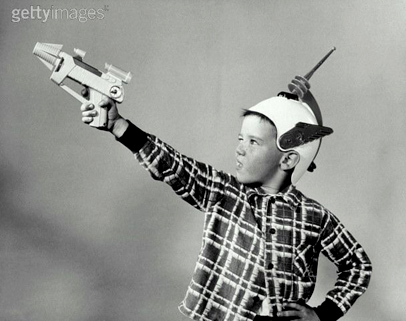
\includegraphics[width=2.0in]{Images/remco_gun_boy2.jpg}}
\item[\redcirc] \highpriority\ \redtext{Interface with Moray}
\pause
\item[$\bigcirc$] \ldots ?
\end{enumerate}
\end{minipage}
\end{center}
\end{frame}

 % What is needed to complete V6.0 (radiation)?
%%======================================================================
\NEWSEC
%======================================================================

\subsection{\ssContribute}

\begin{frame}[fragile,label=ss-contribute] 
\label{frame:help}
\secframetitle{\ssContribute}
\textbf{Thanks for asking!} \\ \ \\
\begin{minipage}{4.5in}
\begin{center}
\rowcolors[]{1}{blue!5}{blue!10}
\begin{tabular}{rl}
\uncover<1->{\orow{\textbf{Beta User}}} &
  \uncover<1->{\orow{download and experiment with \enzop}} \\
  \uncover<2->{\orow{\textbf{Testing}}} &
  \uncover<2->{\orow{develop and submit test problems}} \\
  \uncover<3->{\erow{\textbf{Debugging}}} &
  \uncover<3->{\erow{help track down and fix bugs}} \\
  \uncover<4->{\orow{\textbf{Documentation}}} &
  \uncover<4->{\orow{write or update documentation}} \\
  \uncover<5->{\erow{\textbf{Developing}}} &
  \uncover<5->{\erow{migrate \enzo\ physics capabilities to \enzop }} \\
  \uncover<6->{\erow{\textbf{Refactoring}}} &
  \uncover<6->{\erow{refactor uglier or more complicated code sections}} \\
  \uncover<7->{\orow{\textbf{Managing}}} &
  \uncover<7->{\orow{help direct the development effort}}
 \end{tabular}
\end{center}
\end{minipage} \\

\end{frame}
 % How can I contribute?
%%======================================================================
\NEWSEC
%======================================================================

\subsection{\ssFutureSummary}

%----------------------------------------------------------------------

\begin{frame}[fragile,label=ss-future-summary] 
\secframetitle{\ssFutureSummary}
\begin{itemize}
\item Enzo-P / Cello development entering a new stage
\begin{itemize}
\item pipelined development
\item Enzo-P: new physics capabilities
\item Cello: new framework support
\end{itemize}
\item Requires multiple developers!
\begin{itemize}
\item Dan Reynolds working on scalable gravity
\item More help wanted!
\end{itemize}
\end{itemize}
\vfill
\centerline{$\qed$}
\end{frame}



\end{document}


